%% For double-blind review submission, w/o CCS and ACM Reference (max submission space)
%\documentclass[acmsmall,review,anonymous]{acmart}\settopmatter{printfolios=true,printccs=false,printacmref=false}
%\documentclass[acmsmall]{acmart}\settopmatter{}
%% For editing double-blind review submission, w/o CCS and ACM Reference (max submission space)
\documentclass[acmsmall,review,showframe]{acmart}\settopmatter{printfolios=true,printccs=false,printacmref=false}
%% For double-blind review submission, w/ CCS and ACM Reference
%\documentclass[acmsmall,review,anonymous]{acmart}\settopmatter{printfolios=true}
%% For single-blind review submission, w/o CCS and ACM Reference (max submission space)
%\documentclass[acmsmall,review]{acmart}\settopmatter{printfolios=true,printccs=false,printacmref=false}
%% For single-blind review submission, w/ CCS and ACM Reference
%\documentclass[acmsmall,review]{acmart}\settopmatter{printfolios=true}
%% For final camera-ready submission, w/ required CCS and ACM Reference
%\documentclass[acmsmall]{acmart}\settopmatter{}


%% Journal information
%% Supplied to authors by publisher for camera-ready submission;
%% use defaults for review submission.
% \acmJournal{PACMPL}
% \acmVolume{1}
% \acmNumber{CONF} % CONF = POPL or ICFP or OOPSLA
% \acmArticle{1}
% \acmYear{2018}
% \acmMonth{1}
% \acmDOI{} % \acmDOI{10.1145/nnnnnnn.nnnnnnn}
% \startPage{1}

%% Copyright information
%% Supplied to authors (based on authors' rights management selection;
%% see authors.acm.org) by publisher for camera-ready submission;
%% use 'none' for review submission.
\setcopyright{none}
%\setcopyright{acmcopyright}
%\setcopyright{acmlicensed}
%\setcopyright{rightsretained}
%\copyrightyear{2018}           %% If different from \acmYear
\usepackage[utf8]{inputenc}

%% Bibliography style
\bibliographystyle{ACM-Reference-Format}
%% Citation style
%% Note: author/year citations are required for papers published as an
%% issue of PACMPL.
\citestyle{acmauthoryear}   %% For author/year citations


% %% Some recommended packages.
% \usepackage{booktabs}   %% For formal tables:
%                         %% http://ctan.org/pkg/booktabs
\usepackage{subcaption} %% For complex figures with subfigures/subcaptions
                        %% http://ctan.org/pkg/subcaption
\usepackage{wrapfig}

\usepackage{placeins}

\usepackage{todonotes}

\usepackage{ifthen}
\usepackage{pgf}
\usepackage{ulem}
\usepackage{tikz}
\usepackage{tikzpeople}
\usetikzlibrary{backgrounds}
\usetikzlibrary{fit}
\usetikzlibrary{calc}
\usetikzlibrary{positioning}
\usetikzlibrary{patterns}
\usetikzlibrary{decorations.pathreplacing}
\usetikzlibrary{arrows,shapes}
\usepackage{amssymb}

% Active adversary
\newcommand{\actadv}[4][]{
  \ifthenelse{\equal{#1}{}}{
    \draw[fill=white] #2 rectangle #3 node[pos=.5] {};
    \draw ($#2 + (2.25,1.5)$) node[devil,mirrored,minimum size=1cm] {};
    \draw[fill=white, fill opacity=0.5] #2 rectangle #3 node[pos=.5] {};
    \draw #2 rectangle #3 node[pos=.5,align=center] {\footnotesize #4};
  }{
    \onlyenv<#1>
    \draw[fill=white] #2 rectangle #3 node[pos=.5] {};
    \draw ($#2 + (3,1.5)$) node[devil,mirrored,minimum size=1cm] {};
    \draw[fill=white, fill opacity=0.5] #2 rectangle #3 node[pos=.5] {};
    \draw #2 rectangle #3 node[pos=.5] {\footnotesize #4};
    \endonlyenv
  }
}

% Inactive adversary
\newcommand{\inactadv}[4][]{
  \ifthenelse{\equal{#1}{}}{
    \draw[fill=white] #2 rectangle #3 node[pos=.5] {};
    \draw ($#2 + (2.25,1.5)$) node[devil,mirrored,minimum size=1cm] {};
    \draw[fill=white, fill opacity=0.4] #2 rectangle #3 node[pos=.5] {};
    \draw[fill=gray, fill opacity=0.5] #2 rectangle #3 node[pos=.5] {};
    \draw #2 rectangle #3 node[pos=.5] {\footnotesize #4};
  }{
    \onlyenv<#1>
    \draw[fill=white] #2 rectangle #3 node[pos=.5] {};
    \draw ($#2 + (3,1.5)$) node[devil,mirrored,minimum size=1cm] {};
    \draw[fill=white, fill opacity=0.4] #2 rectangle #3 node[pos=.5] {};
    \draw[fill=gray, fill opacity=0.5] #2 rectangle #3 node[pos=.5] {};
    \draw #2 rectangle #3 node[pos=.5] {\footnotesize #4};
    \endonlyenv
  }
}

% Active stack frame
\newcommand{\actsf}[4][]{
  \ifthenelse{\equal{#1}{}}{
    \draw[fill=white] #2 rectangle #3 node[pos=.5] {\footnotesize #4};
  }{
   \draw<#1>[fill=white] #2 rectangle #3 node[pos=.5] {#4};
 }
}

% Inactive stack frame
\newcommand{\inactsf}[4][]{
  \ifthenelse{\equal{#1}{}}{
    \draw[fill=white] #2 rectangle #3 node[pos=.5] {};
    \draw[fill=gray, fill opacity=0.5] #2 rectangle #3 node[pos=.5] {};
    \draw #2 rectangle #3 node[pos=.5] {\footnotesize #4};
  }{
    \draw<#1>[fill=white] #2 rectangle #3 node[pos=.5] {};
    \draw<#1>[fill=gray, fill opacity=0.5] #2 rectangle #3 node[pos=.5] {};
    \draw<#1> #2 rectangle #3 node[pos=.5] {\footnotesize #4};
  }
}

\newcommand{\capbrace}[3][sp1]{
  \draw [decorate,decoration={brace,amplitude=10pt,mirror,raise=4pt},yshift=0pt]
  #2 -- #3 node[draw=black] (#1) [black,midway,xshift=0.8cm] {};

}

\newcommand{\stdstackstart}{
  \scope
    \clip (-.1,-.1) rectangle (4.6,11.1);
    \fill[fill=white] (0,0) rectangle (4.5,11);
    \draw (0,0) -- (0,11);
    \draw (4.5,0) -- (4.5,11);
    \draw[fill=gray!50] (0,-.5) rectangle (4.5,2)
    node[pos=.5,color=black,align=center,yshift=0.1cm] {\footnotesize Higher
      stack\\\footnotesize frames...};
  \endscope
  % \draw[->] (-2,0) -- node[midway,sloped,above] {stack grows upward} (-2,15);
  \draw (-1.5,0) node {};
  \draw (-1.5,15) node {};
}


% stolen from https://tex.stackexchange.com/questions/14225/is-there-the-easiest-way-to-toggle-show-hide-navigational-grids-in-tikz/14230
\makeatletter
\newif\if@showgrid@grid
\newif\if@showgrid@left
\newif\if@showgrid@right
\newif\if@showgrid@below
\newif\if@showgrid@above
\tikzset{%
    every show grid/.style={},
    show grid/.style={execute at end picture={\@showgrid{grid=true,#1}}},%
    show grid/.default={true},
    show grid/.cd,
    labels/.style={font={\sffamily\small},help lines},
    xlabels/.style={},
    ylabels/.style={},
    keep bb/.code={\useasboundingbox (current bounding box.south west) rectangle (current bounding box.north west);},
    true/.style={left,below},
    false/.style={left=false,right=false,above=false,below=false,grid=false},
    none/.style={left=false,right=false,above=false,below=false},
    all/.style={left=true,right=true,above=true,below=true},
    grid/.is if=@showgrid@grid,
    left/.is if=@showgrid@left,
    right/.is if=@showgrid@right,
    below/.is if=@showgrid@below,
    above/.is if=@showgrid@above,
    false,
}

\def\@showgrid#1{%
    \begin{scope}[every show grid,show grid/.cd,#1]
    \if@showgrid@grid
    \begin{pgfonlayer}{background}
    \draw [help lines]
        (current bounding box.south west) grid
        (current bounding box.north east);
%
    \pgfpointxy{1}{1}%
    \edef\xs{\the\pgf@x}%
    \edef\ys{\the\pgf@y}%
    \pgfpointanchor{current bounding box}{south west}
    \edef\xa{\the\pgf@x}%
    \edef\ya{\the\pgf@y}%
    \pgfpointanchor{current bounding box}{north east}
    \edef\xb{\the\pgf@x}%
    \edef\yb{\the\pgf@y}%
    \pgfmathtruncatemacro\xbeg{ceil(\xa/\xs)}
    \pgfmathtruncatemacro\xend{floor(\xb/\xs)}
    \if@showgrid@below
    \foreach \X in {\xbeg,...,\xend} {
        \node [below,show grid/labels,show grid/xlabels] at (\X,\ya) {\X};
    }
    \fi
    \if@showgrid@above
    \foreach \X in {\xbeg,...,\xend} {
        \node [above,show grid/labels,show grid/xlabels] at (\X,\yb) {\X};
    }
    \fi
    \pgfmathtruncatemacro\ybeg{ceil(\ya/\ys)}
    \pgfmathtruncatemacro\yend{floor(\yb/\ys)}
    \if@showgrid@left
    \foreach \Y in {\ybeg,...,\yend} {
        \node [left,show grid/labels,show grid/ylabels] at (\xa,\Y) {\Y};
    }
    \fi
    \if@showgrid@right
    \foreach \Y in {\ybeg,...,\yend} {
        \node [right,show grid/labels,show grid/ylabels] at (\xb,\Y) {\Y};
    }
    \fi
    \end{pgfonlayer}
    \fi
    \end{scope}
}
\makeatother


 	
%%% Local Variables:
%%% TeX-master: "paper"
%%% End:

% Math packages
\usepackage{amsmath,amsfonts,amssymb,amsthm}
\usepackage{mathrsfs}
\usepackage{thmtools}
\usepackage{array}
\usepackage{cleveref}
\usepackage{stmaryrd}
\usepackage{mathpartir}


% Command control packages
\usepackage{ifthen}
\usepackage{ifpdf}

% Listings
\usepackage{listings}
\lstset{
  basicstyle=\ttfamily,
  columns=fullflexible,
  keepspaces=true,
  mathescape
}


% Tikz
\usepackage{tikz}

%%% Comments
% Comments
\newcommand\lau[1]{{\color{purple} \sf \footnotesize {LS: #1}}\\}
\newcommand\dominique[1]{{\color{purple} \sf \footnotesize {DD: #1}}\\}
\newcommand\lars[1]{{\color{purple} \sf \footnotesize {LB: #1}}\\}

%%% Math environments
\declaretheorem[numbered=yes,name=Lemma,qed=$\blacksquare$]{lemma}
\declaretheorem[numbered=yes,name=Theorem,qed=$\blacksquare$]{theorem}
\declaretheorem[numbered=yes,name=Definition,qed=$\blacksquare$]{definition}
\declaretheorem[numbered=yes,name=Specification,qed=$\blacksquare$]{specification}


%%% Math notation
\newcommand{\defeq}{\stackrel{\textit{\tiny{def}}}{=}}
\newcommand{\defbnf}{::=}
\newcommand{\sem}[1]{\left\llbracket #1 \right\rrbracket}
\newcommand{\ssem}[2][\Phi]{\sem{#2}_{\mathrm{src}}(#1)}
\newcommand{\tsem}[2][\Phi]{\sem{#2}_{\mathrm{trg}}(#1)}
\newcommand{\dom}{\mathrm{dom}}
\newcommand{\powerset}[1]{\mathcal{P}(#1)}

\newcommand{\npair}[2][n]{\left(#1,#2\right)}

\newcommand{\nsubeq}[1][n]{\overset{#1}{\subseteq}}
\newcommand{\nsupeq}[1][n]{\overset{#1}{\supseteq}}
\newcommand{\nequal}[1][n]{\overset{#1}{=}}

% Function arrows
\newcommand{\fun}{\rightarrow}
\newcommand{\parfun}{\rightharpoonup}
\newcommand{\monnefun}{\xrightarrow{\textit{\tiny{mon, ne}}}}



% Text
\newcommand{\tand}{\text{ and }}
\newcommand{\tor}{\text{ or }}
\newcommand{\totherwise}{\text{otherwise }}

% Equivalences
\newcommand{\sconeq}{\mathrel{\src{\approx_{\mathrm{ctx}}}}}
\newcommand{\tconeq}{\mathrel{\approx_{\mathrm{ctx}}}}

%%% Logical Relation notation
\newcommand{\typesetlr}[1]{\mathcal{#1}}
\newcommand{\lre}{\typesetlr{E}}
\newcommand{\lrexj}{\typesetlr{E}_{\var{xjmp}}}
\newcommand{\lrk}{\typesetlr{K}}
\newcommand{\lrr}{\typesetlr{R}}
\newcommand{\lro}{\typesetlr{O}}
\newcommand{\lrv}{\typesetlr{V}}
\newcommand{\lrp}{\typesetlr{P}}
\newcommand{\lrm}{\typesetlr{M}}

\newcommand{\stpair}[3][]{
\ifthenelse{\equal{#1}{}}
{\left(\src{#2_S},#3_T\right)}
{\left(\src{#2},#3\right)}}


\newcommand{\memSat}[3][n]{#2 :_{#1}#3}

\newcommand{\World}{\mathrm{World}}
\newcommand{\RegionName}{\mathrm{RegionName}}
\newcommand{\Region}{\mathrm{Region}}
\newcommand{\spatial}{\mathrm{spatial}}
\newcommand{\spatialo}{\mathrm{spatial\_owned}}
\newcommand{\pure}{\mathrm{pure}}
\newcommand{\revoked}{\mathrm{revoked}}
\newcommand{\State}{\mathrm{State}}
\newcommand{\Rels}{\mathrm{Rels}}
\newcommand{\UPred}[1]{\mathrm(#1)}

\newcommand{\future}{\sqsupseteq}
\newcommand{\pub}{\mathrm{pub}}
\newcommand{\privft}{\future^{\priv}}
\newcommand{\pubft}{\future^{\pub}}
\newcommand{\monprivnefun}{\xrightarrow[\text{\tiny{$\privft$}}]{\textit{\tiny{mon, ne}}}}
\newcommand{\monpubnefun}{\xrightarrow[\text{\tiny{$\pubft$}}]{\textit{\tiny{mon, ne}}}}

%%% Regions
\newcommand{\stdreg}[2]{\iota^{\mathrm{std},#2}_{#1}}
\newcommand{\stareg}[2][\stpair{\ms}{\ms}]{\iota^{\mathrm{sta},#2}_{#1}}
\newcommand{\spa}{\mathrm{s}}
\newcommand{\spao}{\mathrm{so}}
\newcommand{\pur}{\mathrm{p}}

%%% Instruction formatting
\newcommand{\sourcecolortext}{blue}
\newcommand{\sourcecolor}{\color{blue}}
\newcommand{\src}[1]{{\sourcecolor #1}}
\newcommand{\targetcolortext}{black}
\newcommand{\targetcolor}[1]{\color{black}}
\newcommand{\trg}[1]{{\targetcolor{} #1}}

\newcommand{\zinstr}[1]{\texttt{#1}}
\newcommand{\oneinstr}[2]{
  \ifthenelse{\equal{#2}{}}
  {\zinstr{#1}}
  {\zinstr{#1} \; #2}
}
\newcommand{\twoinstr}[3]{
  \ifthenelse{\equal{#2#3}{}}
  {\zinstr{#1}}
  {\zinstr{#1} \; #2 \; #3}
}
\newcommand{\threeinstr}[4]{
  \ifthenelse{\equal{#2#3#4}{}}
  {\zinstr{#1}}
  {\zinstr{#1} \; #2 \; #3 \; #4}
}

\newcommand{\fourinstr}[5]{
  \ifthenelse{\equal{#2#3#4#5}{}}
  {\zinstr{#1}}
  {\zinstr{#1} \; #2 \; #3 \; #4 \; #5}
}


%%% Source language
% No arguments
\newcommand{\sfail}{\zinstr{\src{fail}}}
\newcommand{\shalt}{\zinstr{\src{halt}}}
\newcommand{\sreturn}{\zinstr{\src{return}}}

% One argument
\newcommand{\sjmp}[1]{\oneinstr{\src{jmp}}{#1}}
\newcommand{\spush}[1]{\oneinstr{\src{push}}{#1}}
\newcommand{\spop}[1]{\oneinstr{\src{pop}}{#1}}

% Two arguments
\newcommand{\sjnz}[2]{\twoinstr{\src{jnz}}{#1}{#2}}
\newcommand{\sisptr}[2]{\twoinstr{\src{gettype}}{#1}{#2}}
\newcommand{\sgeta}[2]{\twoinstr{\src{geta}}{#1}{#2}}
\newcommand{\sgetb}[2]{\twoinstr{\src{getb}}{#1}{#2}}
\newcommand{\sgete}[2]{\twoinstr{\src{gete}}{#1}{#2}}
\newcommand{\sgetp}[2]{\twoinstr{\src{getp}}{#1}{#2}}
%\newcommand{\sgetloc}[2]{\twoinstr{\src{getloc}}{#1}{#2}}
\newcommand{\sgetlin}[2]{\twoinstr{\src{get}}{#1}{#2}}
\newcommand{\smove}[2]{\twoinstr{\src{move}}{#1}{#2}}
\newcommand{\sstore}[2]{\twoinstr{\src{store}}{#1}{#2}}
\newcommand{\sload}[2]{\twoinstr{\src{load}}{#1}{#2}}
\newcommand{\scca}[2]{\twoinstr{\src{cca}}{#1}{#2}}
\newcommand{\ssload}[2]{\twoinstr{\src{sload}}{#1}{#2}}
\newcommand{\sxjmp}[2]{\twoinstr{\src{xjmp}}{#1}{#2}}
\newcommand{\ssetatob}[2]{\twoinstr{\src{seta2b}}{#1}{#2}}
% scall - special two instruction
\newcommand{\scall}[4][]{  
\ifthenelse{\equal{#3#4}{}}
  {\ensuremath{\zinstr{\src{call}}_{#1}^{#2}}}
  {\ensuremath{\zinstr{\src{call}}_{#1}^{#2} \; #3 \; #4}}
}


% Three arguments
\newcommand{\srestrict}[3]{\threeinstr{\src{restrict}}{#1}{#2}{#3}}
\newcommand{\slt}[3]{\threeinstr{\src{lt}}{#1}{#2}{#3}}
\newcommand{\splus}[3]{\threeinstr{\src{plus}}{#1}{#2}{#3}}
\newcommand{\sminus}[3]{\threeinstr{\src{minus}}{#1}{#2}{#3}}
\newcommand{\scseal}[3]{\threeinstr{\src{cseal}}{#1}{#2}{#3}}
\newcommand{\ssplice}[3]{\threeinstr{\src{splice}}{#1}{#2}{#3}}


% Four arguments
%\newcommand{\ssubseg}[4]{\fourinstr{\src{subseg}}{#1}{#2}{#3}{#4}}
\newcommand{\ssplit}[4]{\fourinstr{\src{split}}{#1}{#2}{#3}{#4}}

%%% Target language
% No arguments
\newcommand{\tfail}{\zinstr{\trg{fail}}}
\newcommand{\thalt}{\zinstr{\trg{halt}}}

% One argument
\newcommand{\tjmp}[1]{\oneinstr{\trg{jmp}}{#1}}

% Two arguments
\newcommand{\tjnz}[2]{\twoinstr{\trg{jnz}}{#1}{#2}}
\newcommand{\tisptr}[2]{\twoinstr{\trg{gettype}}{#1}{#2}}
\newcommand{\tgeta}[2]{\twoinstr{\trg{geta}}{#1}{#2}}
\newcommand{\tgetb}[2]{\twoinstr{\trg{getb}}{#1}{#2}}
\newcommand{\tgete}[2]{\twoinstr{\trg{gete}}{#1}{#2}}
\newcommand{\tgetp}[2]{\twoinstr{\trg{getp}}{#1}{#2}}
%\newcommand{\tgetloc}[2]{\twoinstr{\trg{getloc}}{#1}{#2}}
\newcommand{\tgetlin}[2]{\twoinstr{\trg{getl}}{#1}{#2}}
\newcommand{\tmove}[2]{\twoinstr{\trg{move}}{#1}{#2}}
\newcommand{\tstore}[2]{\twoinstr{\trg{store}}{#1}{#2}}
\newcommand{\tload}[2]{\twoinstr{\trg{load}}{#1}{#2}}
\newcommand{\tcca}[2]{\twoinstr{\trg{cca}}{#1}{#2}}
\newcommand{\txjmp}[2]{\twoinstr{\trg{xjmp}}{#1}{#2}}
\newcommand{\tsetatob}[2]{\twoinstr{\trg{seta2b}}{#1}{#2}}

% Three arguments
\newcommand{\tsplice}[3]{\threeinstr{\trg{splice}}{#1}{#2}{#3}}
\newcommand{\trestrict}[3]{\threeinstr{\trg{restrict}}{#1}{#2}{#3}}
\newcommand{\tlt}[3]{\threeinstr{\trg{lt}}{#1}{#2}{#3}}
\newcommand{\tplus}[3]{\threeinstr{\trg{plus}}{#1}{#2}{#3}}
\newcommand{\tminus}[3]{\threeinstr{\trg{minus}}{#1}{#2}{#3}}
\newcommand{\tcseal}[3]{\threeinstr{\trg{cseal}}{#1}{#2}{#3}}

% Four arguments
%\newcommand{\tsubseg}[4]{\fourinstr{\trg{subseg}}{#1}{#2}{#3}{#4}}
\newcommand{\tsplit}[4]{\fourinstr{\trg{split}}{#1}{#2}{#3}{#4}}

%%% Domains
\newcommand{\plaindom}[1]{\mathrm{#1}}

\newcommand{\nats}{\mathbb{N}}
\newcommand{\ints}{\mathbb{Z}}

%%% Updates
\newcommand{\update}[2]{[#1 \mapsto #2]}
\newcommand{\updReg}[2]{\update{\reg.#1}{#2}}
\newcommand{\updPc}[1]{\Phi\updReg{\pcreg}{#1}}

%%% Source dom
\newcommand{\shareddom}[1]{\mathrm{#1}}
\newcommand{\RegName}{\shareddom{RegisterName}}
\newcommand{\Addr}{\shareddom{Addr}}
\newcommand{\Seal}{\shareddom{Seal}}
\newcommand{\Perm}{\shareddom{Perm}}
\newcommand{\Caps}{\shareddom{Cap}}
\newcommand{\SealableCaps}{\shareddom{SealableCap}}
\newcommand{\Word}{\shareddom{Word}}
\newcommand{\Instr}{\shareddom{Instr}}
\newcommand{\Mem}{\shareddom{Memory}}
\newcommand{\Reg}{\shareddom{RegisterFile}}
\newcommand{\Stk}{\shareddom{Stack}}
\newcommand{\Conf}{\shareddom{Conf}}
\newcommand{\ExecConf}{\shareddom{ExecConf}}
%\newcommand{\Global}{\shareddom{Global}}
\newcommand{\Linear}{\shareddom{Linear}}
\newcommand{\MemSeg}{\shareddom{MemorySegment}}
\newcommand{\StkFrame}{\shareddom{StackFrame}}
\newcommand{\Stack}{\shareddom{Stack}}

\newcommand{\scbnf}{\shareddom{sc}}
\newcommand{\cbnf}{\shareddom{c}}
\newcommand{\permbnf}{\shareddom{perm}}
\newcommand{\addrbnf}{\shareddom{a}}
\newcommand{\basebnf}{\shareddom{base}}
\newcommand{\aendbnf}{\shareddom{end}}
\newcommand{\rbnf}{\shareddom{r}}
%\newcommand{\glbnf}{\shareddom{gl}}
\newcommand{\linbnf}{\shareddom{l}}
\newcommand{\sealbasebnf}{\sigma_\shareddom{base}}
\newcommand{\sealendbnf}{\sigma_\shareddom{end}}

\newcommand{\sstk}{\shareddom{stk}}
\newcommand{\smsstk}{\shareddom{ms_{stk}}}
\newcommand{\sstkframe}{\shareddom{frame}}
\newcommand{\sopc}{\shareddom{opc}}
\newcommand{\sastk}{\shareddom{a_{stk}}}
\newcommand{\perm}{\var{perm}}
%\newcommand{\gl}{\var{g}}
\newcommand{\lin}{\var{l}}
\newcommand{\base}{\shareddom{base}}
\newcommand{\aend}{\shareddom{end}}
\newcommand{\addr}{\shareddom{a}}
\newcommand{\scap}{\shareddom{c}}
\newcommand{\sms}{\shareddom{ms}}

\newcommand{\stkptr}[1]{\mathrm{stack\text{-}ptr}(#1)}
\newcommand{\retptr}{\mathrm{ret\text{-}ptr}}
\newcommand{\retptrd}{\mathrm{ret\text{-}ptr\text{-}data}}
\newcommand{\retptrc}{\mathrm{ret\text{-}ptr\text{-}code}}

\newcommand{\seal}[1]{\shareddom{seal}(#1)}
\newcommand{\sealed}[1]{\shareddom{sealed}(#1)}

\newcommand{\failed}{\mathrm{failed}}
% DOMI: defining a macro named ``undefined'' breaks many latex packages.
%       (this is just another way that LaTeX is broken as a programming language)
% \newcommand{\undefined}{\mathrm{undefined}}
\newcommand{\tundefined}{\mathrm{undefined}}
\newcommand{\halted}{\mathrm{halted}}

%%% Target domain
\newcommand{\targetdom}[1]{\mathrm{#1}}
\newcommand{\tRegName}{\targetdom{RegisterName}}

%%% Programs and contexts
\newcommand{\program}{\mathscr{P}}
\newcommand{\context}{\mathscr{C}}

\newcommand{\plug}[2]{#1[#2]}

%%% Operational semantics
\newcommand{\step}{\rightarrow}
\newcommand{\nstep}[1][n]{\step_{#1}}
\newcommand{\steps}{\step^*}
\newcommand{\diverge}{{\Uparrow}}
\newcommand{\term}[1][-]{{\Downarrow_{#1}}}

%%% Variables
\newcommand{\var}[1]{\mathit{#1}}
\newcommand{\rn}{\var{rn}}
\newcommand{\reg}{\var{reg}}
\newcommand{\mem}{\var{mem}}
\newcommand{\ms}{\var{ms}}
\newcommand{\pc}{\var{pc}}
\newcommand{\stk}{\var{stk}}
\newcommand{\link}{\var{link}}
\newcommand{\stkf}{\stk_{\var{frame}}}
\newcommand{\ret}{\var{ret}}
\newcommand{\data}{\var{data}}
\newcommand{\code}{\var{code}}
\newcommand{\priv}{\var{priv}}
\newcommand{\opc}{\var{opc}}
\newcommand{\odata}{\var{odata}}
\newcommand{\vsc}{\var{sc}}
\newcommand{\cb}{\vsc}
\newcommand{\baddr}{\var{b}}
\newcommand{\eaddr}{\var{e}}
\newcommand{\aaddr}{\var{a}}
\newcommand{\stdrng}{[\baddr,\eaddr]}

%%% Constants
\newcommand{\constant}[1]{\mathrm{#1}}
\newcommand{\calllen}{\constant{call\_len}}
\newcommand{\stkb}{\constant{stk\_base}}

%%% Named registers
\newcommand{\pcreg}{\mathrm{pc}}
\newcommand{\rstk}{\mathrm{r}_\mathrm{stk}}
\newcommand{\rO}{\mathrm{r}_\mathrm{ret}}
\newcommand{\rret}{\rO}
\newcommand{\rretc}{\mathrm{r}_\mathrm{ret code}}
\newcommand{\rretd}{\mathrm{r}_\mathrm{ret data}}
\newcommand{\rdata}{\mathrm{r}_\mathrm{data}}
\newcommand{\rtmp}[1]{\mathrm{r}_\mathrm{t#1}}



%%% locality
%\newcommand{\plainlocality}[1]{\mathrm{#1}}
%\newcommand{\glob}{\plainlocality{global}}
%\newcommand{\local}{\plainlocality{local}}

%%% linearity
\newcommand{\plainlinearity}[1]{\mathrm{#1}}
\newcommand{\linear}{\plainlinearity{linear}}
\newcommand{\normal}{\plainlinearity{normal}}


%%% Permissions
\newcommand{\plainperm}[1]{\textsc{#1}}
%\newcommand{\rwlx}{\plainperm{rwlx}}
\newcommand{\rwx}{\plainperm{rwx}}
\newcommand{\rx}{\plainperm{rx}}
%\newcommand{\rwlxo}{\plainperm{rwlxo}}
%\newcommand{\rwlo}{\plainperm{rwlo}}
%\newcommand{\rwl}{\plainperm{rwl}}
%\newcommand{\rwxo}{\plainperm{rwxo}}
%\newcommand{\rwo}{\plainperm{rwo}}
\newcommand{\rw}{\plainperm{rw}}
%\newcommand{\rxo}{\plainperm{rxo}}
\newcommand{\readonly}{\plainperm{r}}
\newcommand{\ro}{\readonly}
\newcommand{\noperm}{\plainperm{0}}
%\newcommand{\nopermo}{\plainperm{0o}}
%\newcommand{\enter}{\plainperm{e}}
%\newcommand{\entero}{\plainperm{eo}}

%%% Braces
\newcommand{\comp}[1]{[#1]}

%%% Functions
\newcommand{\plainfun}[2]{
  \ifthenelse{\equal{#2}{}}
  {\mathit{#1}}
  {\mathit{#1}(#2)}
}

%\newcommand{\isLoc}[1]{\plainfun{isLocal}{#1}}
%\newcommand{\nonLoc}[1]{\plainfun{nonLocal}{#1}}
%\newcommand{\opaquePerm}[1]{\plainfun{opaquePerm}{#1}}
%\newcommand{\updPcPerm}[1]{\plainfun{updatePcPerm}{#1}}
%\newcommand{\writeLocalAllowed}[1]{\plainfun{writeLocalAllowed}{#1}}
\newcommand{\addressable}[1]{\plainfun{addressable}{#1}}
\newcommand{\callCond}[1]{\plainfun{callCondition}{#1}}
\newcommand{\decInstr}[1]{\plainfun{decodeInstruction}{#1}}
\newcommand{\decPerm}[1]{\plainfun{decodePerm}{#1}}
\newcommand{\encInstr}[1]{\plainfun{encodeInstruction}{#1}}
\newcommand{\encPerm}[1]{\plainfun{encocePerm}{#1}}
\newcommand{\encLin}[1]{\plainfun{encoceLin}{#1}}
\newcommand{\encType}[1]{\plainfun{encodeType}{#1}}
\newcommand{\exec}[1]{\plainfun{executable}{#1}}
\newcommand{\execCond}[1]{\plainfun{executeCondition}{#1}}
\newcommand{\isLinear}[1]{\plainfun{isLinear}{#1}}
\newcommand{\linCons}[1]{\plainfun{linearityConstraint}{#1}}
\newcommand{\noRetStkMs}[1]{\plainfun{noRetStk_{ms}}{#1}}
\newcommand{\noRetStkReg}[1]{\plainfun{noRetStk_{reg}}{#1}}
\newcommand{\nonExec}[1]{\plainfun{nonExecutable}{#1}}
\newcommand{\nonLinear}[1]{\plainfun{nonLinear}{#1}}
\newcommand{\nonZero}[1]{\plainfun{nonZero}{#1}}
\newcommand{\range}[1]{\plainfun{range}{#1}}
\newcommand{\readAllowed}[1]{\plainfun{readAllowed}{#1}}
\newcommand{\readCond}[1]{\plainfun{readCondition}{#1}}
\newcommand{\writeCond}[1]{\plainfun{writeCondition}{#1}}
\newcommand{\sealAss}[1]{\plainfun{sealAssignment}{#1}}
\newcommand{\updPcAddr}[1]{\plainfun{updatePc}{#1}}
\newcommand{\withinBounds}[1]{\plainfun{withinBounds}{#1}}
\newcommand{\writeAllowed}[1]{\plainfun{writeAllowed}{#1}}
\newcommand{\xjumpResult}[3]{\plainfun{xjumpResult}{#1,#2,#3}}

% Paper specific redefinitions of commands
\renewcommand{\npair}[2][n]{#2}
\renewcommand{\MemSeg}{\shareddom{MemSeg}}
\renewcommand{\Reg}{\shareddom{RegFile}}
\renewcommand{\RegName}{\shareddom{RegName}}
\renewcommand{\decInstr}[1]{\plainfun{decode}{#1}}
\renewcommand{\updPcAddr}[1]{\plainfun{updPc}{#1}}
\renewcommand{\linCons}[1]{\plainfun{linClear}{#1}}
\renewcommand{\nonExec}[1]{\plainfun{nonExec}{#1}}
\renewcommand{\perm}{\var{p}}
\renewcommand{\SealableCaps}{\shareddom{Sealables}}
\renewcommand{\Cap}{\shareddom{NatTok}}
\renewcommand{\rretc}{\mathrm{r}_{\mathrm{rcode}}}
\renewcommand{\rretd}{\mathrm{r}_{\mathrm{rdata}}}
\renewcommand{\comp}{\var{comp}}
\renewcommand{\memSatStack}[3][n]{\npair[#1]{#2} \in \typesetlr{S}(#3)}
\renewcommand{\memSatFStack}[3][n]{\npair[#1]{#2} \in \typesetlt{F}(#3)}
\renewcommand{\Worlds}{\World_{\mathrm{call\_stack}}}
\renewcommand{\Worldfs}{\World_{\mathrm{free\_stack}}}

\renewcommand{\lre}[1][]{\typesetlr{E}^{#1}}
\renewcommand{\lretrusted}[1][]{\lreg[#1]{\trusted}}
\renewcommand{\lrexj}[1][]{\typesetlr{E}^{#1}_{\mathrm{xjmp}}}
\renewcommand{\lrk}[1][]{\typesetlr{K}^{#1}}
\renewcommand{\lrrg}[2][]{\typesetlr{R}^{#1}_{#2}}
\renewcommand{\lrr}[1][]{\lrrg[#1]{\untrusted}}
\renewcommand{\lrrtrusted}[1][]{\lrrg[#1]{\trusted}}
\renewcommand{\lro}[1][]{\typesetlr{O}^{#1}}
\renewcommand{\lrol}{\lro[\preceq,(\ta,\stkb,\gsigrets,\gsigcloss)]}
\renewcommand{\lror}{\lro[\succeq,(\ta,\stkb,\gsigrets,\gsigcloss)]}
\renewcommand{\lrvg}[2][]{\typesetlr{V}^{#1}_{#2}}
\renewcommand{\lrv}[1][]{\lrvg[#1]{\untrusted}}
\renewcommand{\lrvtrusted}[1][]{\lrvg[#1]{\trusted}}
\renewcommand{\lrp}{\typesetlr{P}}

\renewcommand{\lrrs}{\typesetlr{R}}
\renewcommand{\lrm}{\typesetlr{M}}
\renewcommand{\lrcomp}[1][]{\typesetlr{C}^{#1}}
\renewcommand{\lrec}[1][]{\typesetlr{EC}^{#1}}
\renewcommand{\lrheap}[1][]{\typesetlr{H}^{#1}}

\renewcommand{\memSat}[3][]{\memSatGeneric{#1}{#2}{#3}{}}
\renewcommand{\stdreg}[3][]{\iota^{\mathrm{std},#3,#1}_{#2}}
\renewcommand{\stareg}[2][\stpair{\ms}{\ms}]{\iota^{\mathrm{sta},#2}_{#1}}
\renewcommand{\codereg}[2][\mathrm{code}]{\iota^{#1}_{#2}}
\renewcommand{\staureg}[2][\stpair{\ms}{\ms}]{\iota^{\mathrm{sta,\lrv},#2}_{#1}}

\newcommand{\xjmpres}[1]{\plainfun{xjmpRes}{#1}}
\newcommand{\srcxjmpres}[1]{\plainfun{\srcalt{xjmpRes}}{#1}}
\newcommand{\wdjud}[2][ ]{#1 \vdash #2}

\newcommand{\trgcm}{\textsc{LCM}}
\newcommand{\srccm}{\textsc{oLCM}}
\newcommand{\extend}[1]{}

\begin{document}

%% Title information
\title{\stktokens{}: Enforcing Well-bracketed Control Flow and Stack Encapsulation using Linear Capabilities}
% \titlenote{with title note}
% \subtitle{Fully abstract overlay semantics}
% \subtitlenote{with subtitle note}

%% Author information
%% Contents and number of authors suppressed with 'anonymous'.
%% Each author should be introduced by \author, followed by
%% \authornote (optional), \orcid (optional), \affiliation, and
%% \email.
%% An author may have multiple affiliations and/or emails; repeat the
%% appropriate command.
%% Many elements are not rendered, but should be provided for metadata
%% extraction tools.

\author{Lau Skorstengaard}
% \orcid{nnnn-nnnn-nnnn-nnnn}             %% \orcid is optional
\affiliation{
  \institution{Aarhus~University}
  \country{Denmark}                    %% \country is recommended
}
\email{lask@cs.au.dk}

%% Author with two affiliations and emails.
\author{Dominique Devriese}
\orcid{0000-0002-3862-6856}             %% \orcid is optional
\affiliation{
  \institution{Vrije~Universiteit~Brussel}           %% \institution is required
  \country{Belgium}                   %% \country is recommended
}
\email{dominique.devriese@vub.be}         %% \email is recommended

\author{Lars Birkedal}
% \orcid{nnnn-nnnn-nnnn-nnnn}             %% \orcid is optional
\affiliation{
  \institution{Aarhus~University}
  \country{Denmark}                    %% \country is recommended
}
\email{birkedal@cs.au.dk}

\begin{abstract}
  We propose and study \stktokens{}: a new calling convention that provably enforces well-bracketed control flow and local state encapsulation on a capability machine.
  The calling convention is based on linear capabilities: a type of capabilities that are prevented from being duplicated by the hardware.
  In addition to designing and formalizing this new calling convention, we also contribute a new way to formalize and prove that it effectively enforces well-bracketed control flow and local state encapsulation using what we call a fully abstract overlay semantics.
\end{abstract}


% %% 2012 ACM Computing Classification System (CSS) concepts
% %% Generate at 'http://dl.acm.org/ccs/ccs.cfm'.
% \begin{CCSXML}
% <ccs2012>
% <concept>
% <concept_id>10011007.10011006.10011008</concept_id>
% <concept_desc>Software and its engineering~General programming languages</concept_desc>
% <concept_significance>500</concept_significance>
% </concept>
% <concept>
% <concept_id>10003456.10003457.10003521.10003525</concept_id>
% <concept_desc>Social and professional topics~History of programming languages</concept_desc>
% <concept_significance>300</concept_significance>
% </concept>
% </ccs2012>
% \end{CCSXML}

% \ccsdesc[500]{Software and its engineering~General programming languages}
% \ccsdesc[300]{Social and professional topics~History of programming languages}
%% End of generated code


\keywords{fully abstract compilation, secure compilation, capability machines, linear capabilities, well-bracketed control flow, stack frame encapsulation, overlay semantics}


\maketitle


\section{Introduction}
\label{sec:introduction}
\todo[inline]{TODOS ENABLED!!!}
\todo[inline]{Lau: for camera ready version update reference to technical report (and upload the technical report).}
\todo[inline]{Lau: for camera ready version take a look at the coloring in the paper}
\todo[inline]{Lau: for camera ready version if TOPLAS paper accepted, update the reference in LR section. }
Secure compilation is an active topic of research (e.g.~\citep{devriese_modular_2017,patrignani_hyper_2017,abate_good_components_2018,new_universal_embedding_2016,juglaret_beyond_2016}), but a real secure compiler is yet to be made.
Secure compilers preserve source-language (security-relevant) properties even when the compiled code interacts with arbitrary target-language components.
Generally, properties that hold in the source language but not in the target language need to be somehow enforced by the compiler.
Two properties that hold in many high-level source languages, but not in the assembly languages they are compiled to, are well-bracketed control flow and encapsulation of local state.

Well-bracketed control flow (WBCF) expresses that invoked functions must either return to their callers, invoke other functions themselves or diverge, and generally holds in programming languages that do not offer a primitive form of continuations. 
At the assembly level, this property does not hold immediately. 
Invoked functions get direct access to return pointers that they are supposed to jump to a single time at the end of their execution.
There is, however, no guarantee that untrusted assembly code respects this intended usage.
In particular, a function may invoke return pointers from other stack frames than its own: either frames higher in the call stack or ones that no longer exist as they have already returned. 

Local state encapsulation (LSE) is the guarantee that when a function invokes another function, its local variables (saved on its stack frame) will not have been read or modified when the invoked function returns.
At the assembly level, this property also does not hold immediately.
The calling function's local variables are stored on the stack during the invocation, and functions are not supposed to touch stack frames other than their own.
However, untrusted assembly code is free to ignore this requirement and read or overwrite the local state of other stack frames.
To enforce these properties, target language security primitives are needed that can be used to prevent untrusted code from misbehaving without imposing too much overhead on well-behaved code.
The virtual-memory based security primitives on commodity processors do not seem sufficiently fine-grained to efficiently support this.
More suitable security primitives are offered by a type of CPUs known as capability machines \citep{levy_capability-based_1984,watson_cheri:_2015}.
These processors use tagged memory to enforce a strict separation between integers and {\itshape capabilities}: pointers that carry authority.
Capabilities come in different flavours.
Memory capabilities allow reading from and writing to a block of memory.
Additionally, capability machines offer some form of {\itshape object capabilities} that represent low-level encapsulated closures, i.e. a piece of code coupled with private state that it gains access to upon invocation.
The concrete mechanics of object capabilities vary between different capability machines.
% KJAA: This 'sealed' and 'common seal' business is unclear to me.
For example, on a recent capability machine called CHERI they take the form of pairs of capabilities that represent the code and data parts of the closure.
Each of the two capabilities are sealed with a common seal which make them opaque.
The hardware transparently unseals the pair upon invocation~\citep{watson_capability_2015,watson_fast_2016}.

To enforce WBCF and LSE on a capability machine, there are essentially two approaches.
A first approach uses separate stacks for mutually distrusting components, and a central, trusted stack manager component that mediates cross-component invocations.
This idea has been applied in CheriBSD (an operating system built on CHERI)~\citep{watson_capability_2015}, but it is not without downsides.
First, it scales poorly to large amounts of components because of the need to reserve separate stack space for all components.
Also in the presence of higher-order values (e.g. function pointers, objects etc.), the stack manager needs to be able to decide which component a higher-order value belongs to in order to provide it the right stack pointer upon invocation.
It is not clear how this can be done efficiently in the presence of large amounts of components.
Finally, this approach does not allow passing stack references between components.

A more scalable approach retains a single stack shared between components.
Enforcing WBCF and LSE in this approach requires a way to temporarily provide stack and return capabilities to an untrusted component and to revoke them after it returns.
While capability revocation is expensive in general, some capability machines offer restricted forms of revocation that can be implemented efficiently.
For example, CHERI offers a form of {\itshape local} capabilities that can only be stored in registers or on the stack but not in other parts of memory.
\citet{skorstengaard_reasoning_2017} have demonstrated that by making the stack and return pointer local, and by introducing a number of security checks and measures, the two properties can be guaranteed.
In fact, a similar system was envisioned in earlier work on CHERI~\citep{watson2012cheri}. 
% KJAA: 'Boundary crossing' is new here.
However, a problem with this approach is that revoking the local stack and return capabilities on every security boundary crossing requires clearing the entire unused part of the stack, an operation that may be prohibitively expensive.

In this work, we propose and study \stktokens{}: an alternative calling convention that enforces WBCF and LSE with a single shared stack.
Instead of CHERI's local capabilities, it builds on {\itshape linear} capabilities; a new form of capabilities that has not been previously described in the published literature.\footnote{Although they have been mentioned in some technical documents.}
% KJAA: Perhaps make it clear by who and when/where?
The hardware prevents these capabilities from being duplicated.
We propose to make stack and return pointers linear and require components to hand them out in cross-component invocations and to return them in returns.
The non-duplicability of linear capabilities together with some security checks allow us to guarantee WBCF and LSE without large overhead on boundary crossings and in particular without the need for clearing large blocks of memory.

A second contribution of this work is the way in which we formulate these two properties: although the terms ``well-bracketed control flow'' and ``local state encapsulation'' sound precise, it is actually far from clear what they mean, and how best to formalize them.
Formulations in previous work are either partial and not suitable for reasoning~\cite{abadi_control-flow_2005} or lacked evidence of generality~\cite{skorstengaard_reasoning_2017}.
We propose a new formulation using a technique we call {\itshape fully abstract overlay semantics}.
Our new formulation starts from the premise that security results for a calling convention should be reusable as part of a larger proof of a secure compiler.
To accommodate this, we define a second operational semantics for our target language with a native well-bracketed call stack and primitive ways to do calls and returns.
This well-behaved semantics guarantees WBCF and LSE natively for components using our calling convention.
As such, these components can be sure that they will only ever interact with other well-behaved components that respect our desired properties.
To express security of our calling convention, we then show that considering the same components in the original semantics does not give adversaries additional ways to interact with them. 
More formally, we show that mapping a component in the well-behaved semantics to the same component in the original semantics is fully abstract~\cite{abadi_protection_1999}, i.e. that components are indistinguishable to arbitrary adversaries in the well-behaved language iff they are indistinguishable to arbitrary adversaries in the original language.

Compared to~\citet{skorstengaard_reasoning_2017} that prove LSE and WBCF for a handful of examples,
this approach expresses what it means to enforce the desirable properties in a general way and makes it clear that we can support a very general class of programs.
Additionally, formulating security of a calling convention in this way makes it potentially reusable in a larger security proof of a full compiler.
The idea is that security of such a compiler could be verified by proving fully abstract compilation with respect to the well-behaved semantics of the target language, so that the proof can rely on native well-bracketedness and local stack frame encapsulation.
This independent result could then be composed with our result to obtain security of the compiler targeting the real target language, by transitivity of full abstraction.

%The main contributions of this paper are (1) \stktokens{} a calling convention that uses linear capabilities to provably secure LSE and WBCF, and (2) a novel proof technique that we call fully-abstract overlay semantics which we apply to prove the properties of \stktokens{}.
In this paper, we make the following contributions:
% Presents the first formal model of a capability machine with linear capabilities (Section 2)
% Presents a calling convention called \stktokens{} that provably guarantee local state encapsulation and well-bracketed control flow (Section 3)
% Presents a novel proof technique that we call fully-abstract overlay semantics. (Section 4-5)
\begin{itemize}
\item We present \trgcm{}: A formalization of a simple CHERI-like capability machine with linear capabilities (Section~\ref{sec:cap-mach-w-seal-and-lin}).
\item We present a new calling convention \stktokens{} that provably guarantees LSE and WBCF on \trgcm{} (Section~\ref{sec:stktokens-explained}).
\item We present a new way to formalize these guarantees based on a novel
  technique called \textit{fully-abstract overlay semantics} and we prove LSE
  and WBCF claims. This includes:
  \begin{itemize}
  \item defining \srccm{}: an overlay semantics for \trgcm{} with built-in LSE and WBCF (Section~\ref{sec:form-secur-with})
  \item proving full-abstraction for the embedding of \srccm{} into \trgcm{} (Section~\ref{sec:fa-proof}) by
  \item using and defining a cross-language, step-indexed, Kripke logical relation with recursive worlds (Section~\ref{sec:fa-proof}).
  \end{itemize}
\end{itemize}
This paper is accompanied by a technical report~\citep{technical_report} with the elided details and proof.

%\paragraph{Outline} Blabla

% \begin{acks}                            %% acks environment is optional
%                                         %% contents suppressed with 'anonymous'
%   %% Commands \grantsponsor{<sponsorID>}{<name>}{<url>} and
%   %% \grantnum[<url>]{<sponsorID>}{<number>} should be used to
%   %% acknowledge financial support and will be used by metadata
%   %% extraction tools.
%   This material is based upon work supported by the
%   \grantsponsor{GS100000001}{National Science
%     Foundation}{http://dx.doi.org/10.13039/100000001} under Grant
%   No.~\grantnum{GS100000001}{nnnnnnn} and Grant
%   No.~\grantnum{GS100000001}{mmmmmmm}.  Any opinions, findings, and
%   conclusions or recommendations expressed in this material are those
%   of the author and do not necessarily reflect the views of the
%   National Science Foundation.
% \end{acks}

\section{A Capability Machine with Sealing and Linear Capabilities}
\label{sec:cap-mach-w-seal-and-lin}
% Brief intro to section and this cap machine:
% Cap machine inspired by CHERI, but with linear capabilities
In this section, we introduce a simple but representative capability machine with linear capabilities, that we call \trgcm{} (Linear Capability Machine).
\trgcm{} is mainly inspired by CHERI~\citep{watson_cheri:_2015} with linear capabilities as the main addition.
For simplicity, \trgcm{} assumes an infinite address space and unbounded integers.
% \lau{Do we have a good reason to assume an infinite address space for this work?
%   We do not model malloc, so we do not need to worry about what happens when malloc runs out of memory.}

%%% Capabilities
The concept of a capability is the cornerstone of any capability machine.
In its simplest form, a capability is a permission and a range of authority.
The permission dictates the operations the capability can be used for, and the range of authority specifies the range of memory it can act upon.
% Permissions and Range of authority
The capabilities on \trgcm{} are of the form $((\var{perm},\var{lin}),\var{base},\var{end},\var{addr})$ (defined in Figure~\ref{fig:target-syntax} with the rest of the syntax of \trgcm{}). Here $\var{perm}$ is the permission, and $[\var{base},\var{end}]$ is the range of authority.
The available permissions are read-write-execute ($\rwx$), read-write ($\rw$), read-execute ($\rx$), read-only ($\ro$), and null-permission ($\noperm$) ordered by $\le$ as illustrated in Figure~\ref{fig:perm-hier}.
% Pointer and linearity
In addition to the permission and range, capabilities also have a current address $\var{addr}$ and a linearity $\var{lin}$.
The linearity is either $\normal$ for traditional capabilities or $\linear$ for linear ones.
% What is linear capabilities, split/splice
A linear capability is a capability that cannot be duplicated.
This is enforced dynamically on the capability machine, so when a linear capability is moved between registers or memory, the source is cleared.
The non-duplicability of linear capabilities means that a linear capability cannot become aliased if it wasn't to begin with.
\begin{wrapfigure}{r}{0.26\linewidth}
  \centering
  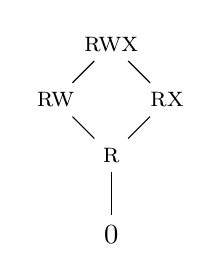
\begin{tikzpicture}[main node/.style={}]
    \node[main node] (rwx) {$\rwx$};
    \node[main node] (rx) [below right of=rwx] {$\rx$};

    \node[main node] (rw) [below left of=rwx,] {$\rw$};
    \node[main node] (r) [below right of=rw] {$\readonly$};
    \node[main node] (0) [below of=r] {$\noperm$};

    \path[every node/.style={font=\sffamily\small}]

    (rw) edge (r)
    (r) edge (0)

    (rwx) edge (rx)

    (rw) edge (rwx)
    (r) edge (rx);
  \end{tikzpicture}

  \caption{Permission hierarchy}
  \label{fig:perm-hier}
\end{wrapfigure}

%%% Seals
% KJAA: Here I am still missing an intuition of what a seal 'is' -- why the range, why the seal as an 'entity'?

Any reasonable capability machine needs a way to set up boundaries between security domains with different authorities.
It also must have a way to cross these boundaries such that (1) the security domain we move from can encapsulate and later regain its authority and (2) the security domain we move to regains all of its authority. 
%The M-Machine~\citep{Dally1997Memo59} inspired capability machine in \citet{skorstengaard_reasoning_2017} uses enter-capabilities to achieve this.
On \trgcm{} we have CHERI-like sealed capabilities to achieve this~\cite{watson_cheri:_2015}.
% seals
A sealed capability makes an underlying capability opaque which means that the underlying capability cannot be changed or used for the operations it normally gives permission to.
In other words, the authority the underlying capability represents is encapsulated under the seal.
Syntactically, the sealed capability is represented as $\sealed{\sigma,\vsc}$ where $\vsc$ is a sealable and $\sigma$ is the seal used to seal the capability.
In order to seal a sealable, it is necessary to have the right to do so.
The right to make sealed capabilities is represented by a sets of seals $\seal{\sigma_\var{base},\sigma_\var{end},\sigma}$.
A set of seal gives the right to seal sealables under seals in the range $[\sigma_\var{base},\sigma_\var{end}]$.
In spirit of the memory capabilities, a set of seals has an active seal $\sigma$ which is the seal currently used to make sealed capabilities.
On \trgcm{}, we represent seals in sets rather than single seals to have a more compact representation of multiple seals and make it possible to have seal allocation (not described here).
As we will see later, sealed capabilities can be unsealed with an \texttt{xjmp}.
When underlying capabilities are unsealed with \texttt{xjmp}, control will be transferred to one of the underlying capability which allows the capability-sealer to decide how the sealed capabilities are used.
The \texttt{xjmp} instruction will be explained in more detail later.
The combination of sealed capabilities and \texttt{xjmp} gives (1) and (2).
\begin{figure}[tb]
  \centering
  \[
  \arraycolsep=1.4pt
  \begin{array}{rrcl l rrcl}
   \addrbnf,\basebnf \in & \Addr & \defeq & \nats & \phantom{mak} & \sealbasebnf, \sigma \in & \Seal & \defeq & \nats\\
    \aendbnf \in & & & \Addr \cup \{\infty \} & & \sealendbnf \in & & & \Seal \cup \{\infty \}\\
    \permbnf \in& \Perm & \defbnf & \rwx \mid \rx \mid \rw \mid \ro \mid \noperm & & &\linbnf & \defbnf & \linear \mid \normal\\
    \vsc \in &\SealableCaps&\defbnf & \multicolumn{6}{l}{((\permbnf,\linbnf),\basebnf,\aendbnf,\addrbnf) \mid \seal{\sealbasebnf,\sealendbnf,\sigma}}\\
    c \in&\Caps& \defbnf &  \SealableCaps \mid \sealed{\sigma,\scbnf} & & w \in &\Word & \defeq & \ints \uplus \Caps\\ 
    r \in& \RegName & \defbnf & \multicolumn{6}{l}{\pcreg \mid \rretd \mid \rretc \mid \rstk \mid \rdata \mid \rtmp{1} \mid \rtmp{2} \mid \dots} \\
    \reg \in &\Reg & \defeq & \RegName \fun \Word & & \mem \in&\Mem & \defeq & \Addr \fun \Word\\
\ms \in  &\MemSeg & \defeq & \Addr \parfun \Word & & \Phi \in & \ExecConf & \defeq & \Mem \times \Reg\\
    &\Conf & \defeq & \multicolumn{6}{l}{\ExecConf \cup \{\failed\} \cup \{\halted\} }
  \end{array}
\]
\[
  \arraycolsep=1.4pt
\begin{array}{rcl}
\multicolumn{3}{l}{    \arraycolsep=0pt
      \com{r} \in  \tRegName \hspace{2.5cm}   \com{\rn} \defbnf \com{r} \mid \nats
}\\
  \Instr &\defbnf & \tjmp{\com{r}} \mid \tjnz{\com{r}}{\com{\rn}} \mid \tmove{\com{r}}{\com{\rn}} \mid \tload{\com{r}}{\com{r}} \mid \tstore{\com{r}}{\com{r}} \mid \tplus{\com{r}}{\com{\rn}}{\com{\rn}} \mid \tminus{\com{r}}{\com{\rn}}{\com{\rn}} \mid\\
         & & \tlt{\com{r}}{\com{\rn}}{\com{\rn}} \mid \tisptr{\com{r}}{\com{r}} \mid\tgetp{\com{r}}{\com{r}} \mid \tgetlin{\com{r}}{\com{r}} \mid \tgetb{\com{r}}{\com{r}} \mid \tgete{\com{r}}{\com{r}} \mid \tgeta{\com{r}}{\com{r}}  \mid \\
  & & \tcca{\com{r}}{\com{n\rn}} \mid \tsetatob{\com{r}} \mid \trestrict{\com{r}}{\com{\rn}} \mid \tcseal{\com{r}}{\com{r}} \mid \txjmp{\com{r}}{\com{r}} \mid  \tsplit{\com{r}}{\com{r}}{\com{r}}{\com{\rn}} \mid\\ 
      & & \tsplice{\com{r}}{\com{r}}{\com{r}} \mid \tfail \mid \thalt 
\end{array}
\]
  \caption{The syntax of our capability machine with seals and linear capabilities.}
  \label{fig:target-syntax}
\end{figure}

%%% Domains
Words on \trgcm{} are capabilities and data (represented by $\ints$).
We assume a finite set of register names $\RegName$ containing at least $\pcreg$, $\rretd$, $\rretc$, $\rstk$, $\rdata$, $\rtmp{1}$, and $\rtmp{2}$, and we define register files as functions from register names to words.
We have complete memories mapping all addresses to words and memory segments mapping some addresses to words (i.e.\ partial functions).
$\trgcm{}$ has two terminated configurations $\halted$ and $\failed$ that respectively signify a successful execution and an execution where something went wrong, e.g.\ an out-of-bounds memory access.
An executable configuration is a register file and memory pair.

\begin{figure}[p]
  \centering
  \begin{mathpar}
    \inference{\Phi(\pcreg) = ((\perm,\_),\baddr,\eaddr,\aaddr) \\
        \baddr \le \aaddr \le \eaddr \and \perm \in \{\rwx,\rx\}
 }{ \Phi \step \sem{\decInstr{\Phi.\mem(\aaddr)}}(\Phi) }
              \and
              \inference{ \forall \Phi' \neq \failed \ldotp \Phi \nrightarrow \Phi'}
                        {\Phi \step \failed }
  \end{mathpar}
  \[
    \begin{array}{l}
  %   \Phi \step
  % \begin{cases}
  %   \sem{\decInstr{\Phi.\mem(\aaddr)}}(\Phi) &
  %   \arraycolsep=0pt
  %     \begin{array}[t]{l}
  %       \text{if }\Phi(\pcreg) = ((\perm,\_),\baddr,\eaddr,\aaddr) \wedge
  %       \baddr \le \aaddr \le \eaddr \wedge \perm \in \{\rwx,\rx\}
  %     \end{array} \\
  %     \failed & \totherwise
  % \end{cases}\\
  \updPcAddr{\Phi} =
  \begin{cases}
    \Phi\updReg{\pcreg}{w} & \Phi(\pcreg) = ((\perm,\lin),\baddr,\eaddr,\aaddr) \wedge w = ((\perm,\lin),\baddr,\eaddr,\aaddr+1)\\
    \Phi  & \totherwise
  \end{cases}\\
  \linCons{w} =
  \begin{cases}
    0 & \isLinear{w} \\
    w & \totherwise
  \end{cases}\\
  \xjmpres{c_1,c_2,\Phi} =
  \begin{cases}
    \Phi\updReg{\pcreg}{c_1}\updReg{\rdata}{c_2} & \nonExec{c_2} \\
    \failed & \totherwise
  \end{cases}
  \end{array}
\]
  \begin{tabular}{|>{$}c<{$}|>{$}p{3.7cm}<{$}|>{\raggedright\arraybackslash}p{6.7cm}|}
    \hline
    i \in \Instr                                 & \sem{i}(\Phi) & Conditions\\
    \hline
    \halt                                        & \halted & \\
    \hline
    \fail                                        & \failed & \\
    % \hline
    % \move{r}{\rn}                                & \updPcAddr{\Phi\updReg{r}{\rn}} & $\rn \in \ints$\\
    \hline
    \move{r}{\rn}                                & \updPcAddr{}\arraycolsep=0pt\array[t]{rl}(\Phi&\updReg{\rn}{w_2}\\ & \updReg{r}{w_1})\endarray & $\rn \in \RegName$ and $w_1 = \Phi(\rn)$ and $w_2 = \linCons{\Phi(\rn)}$ \\
    \hline
    \load{r_1}{r_2}                              & \updPcAddr{}\arraycolsep=0pt\array[t]{rl}(\Phi&\updReg{r_1}{w_1}\\ &\update{\mem.\aaddr}{w_\aaddr})\endarray & $\Phi(r_2) = ((\perm,\_),\baddr,\eaddr,\aaddr)$ and $\baddr \le \aaddr \le \eaddr$ and $\perm \in \{\rwx,\rw,\rx,\ro\}$ and $w_1 = \Phi.\mem(\aaddr)$ and $\isLinear{w_1} \Rightarrow \perm \in \{\rwx,\rw\}$ and $w_a = \linCons{w_1}$\\
    \hline
    \store{r_1}{r_2}                             & \updPcAddr{}\arraycolsep=0pt\array[t]{rl}(\Phi&\updReg{r_2}{w_2}\\ & \update{\mem.\aaddr}{\Phi(r_2)})\endarray & $\Phi(r_1) = ((\perm,\_),\baddr,\eaddr,\aaddr)$ and $\perm \in \{\rwx,\rw\}$ and $\baddr \le \aaddr \le \eaddr$ and $w_2 = \linCons{\Phi(r_2)}$\\
    \hline
    \geta{r_1}{r_2}                              & \updPcAddr{\Phi\updReg{r_1}{w}} & If $\Phi(r_2) = ((\_,\_),\_,\_,\aaddr)$ or $\Phi(r_2) = \seal{\_,\_,\aaddr}$, then $w = \aaddr$ and otherwise $w = -1$\\
    \hline
    \cca{r}{\rn}                                 &\updPcAddr{\Phi\updReg{r}{w}} & $\Phi(\rn) = n \in \ints$ and either $\Phi(r) = ((\perm,\lin),\baddr,\eaddr,\aaddr)$ or $\Phi(r) = (\sigma_\baddr,\sigma_\eaddr,\sigma)$ and $w = ((\perm,\lin),\baddr,\eaddr,\aaddr + n)$ or $w = (\sigma_\baddr,\sigma_\eaddr,\sigma+n)$, respectively \\
    \hline
    \jmp{r}    &\Phi\arraycolsep=0pt\array[t]{l}\updReg{r}{w}\\\updReg{\pcreg}{\Phi(r)}\endarray & $w = \linCons{\Phi(r)}$\\
    \hline
    \xjmp{r_1}{r_2}                              & \Phi' & $\Phi(r_1) = \sealed{\sigma,c_1}$ and $\Phi(r_2) = \sealed{\sigma,c_2}$ and $w_1 = \linCons{c_1}$ and $w_2 = \linCons{c_2}$ and $\Phi' = \xjmpres{c_1,c_2,\Phi\updReg{r_1,r_2}{w_1,w_2}}$  \\
    \hline
    \tsplit{r_1}{r_2}{r_3}{\rn}                  & \updPcAddr{}\arraycolsep=0pt\array[t]{rl}(\Phi&\updReg{r_3}{w}\\ &\updReg{r_1}{c_1}\\ &\updReg{r_2}{c_2})\endarray & $\Phi(r_3) = ((\perm,\lin),\baddr,\eaddr,\aaddr)$ and $\Phi(\rn) = n \in \nats$ and $\baddr \le n < \eaddr$ and $c_1 = ((\perm,\lin),\baddr,n,\aaddr)$ and $c_2 = ((\perm,\lin),n+1,\eaddr,\aaddr)$ and $w = \linCons{\Phi(r_3)}$\\
    \hline
    \splice{r_1}{r_2}{r_3}                       & \updPcAddr{}\arraycolsep=0pt\array[t]{rl}(\Phi&\updReg{r_2}{w_2}\\ &\updReg{r_3}{w_3}\\ &\updReg{r_1}{c})\endarray& $\Phi(r_2) = ((\perm,\lin),\baddr,n,\_)$ and $\Phi(r_3) = ((\perm,\lin),n+1,\eaddr,\aaddr)$ and $\baddr \le n < \eaddr$ and $c = ((\perm,\lin),\baddr,\eaddr,\aaddr)$ and $w_2,w_3 = \linCons{\Phi(r_2),\Phi(r_3)}$\\
    \hline
    \cseal{r_1}{r_2}                             & \updPcAddr{\Phi\updReg{r_1}{\vsc}} & $\Phi(r_1) \in \SealableCaps$ and $\Phi(r_2) = \seal{\sigma_\baddr,\sigma_\eaddr,\sigma}$ and $\sigma_\baddr \le \sigma \le \sigma_\eaddr$ and $\vsc = \sealed{\sigma,\Phi(r_1)}$ \\
    \hline
    \multicolumn{3}{|c|}{\dots} \\
    \hline
    \_                                           & \failed & \totherwise \\
    \hline
  \end{tabular}
\caption{An excerpt of the operational semantics of \trgcm{}}
  \label{fig:target-op-sem}
\end{figure}
% syntax (instructions)
\trgcm{}'s instruction set is somewhat basic with the instructions one expects on most low-level machine as well as capability-related instructions.
The standard instructions are: unconditional and conditional jump (\texttt{jmp} and \texttt{jnz}), copy between registers (\texttt{move}), instructions that load from memory and store to memory (\texttt{load} and \texttt{store}), and arithmetic operations (\texttt{plus}, \texttt{minus}, and \texttt{lt}).
The simplest of the capability instructions inspect the properties of capabilities: type (\texttt{gettype}), linearity (\texttt{getl}), range (\texttt{getb} and \texttt{gete}), current address or seal (\texttt{geta}) or permission (\texttt{getp}).
The current address (or seal) of a capability (or set of seals) can be shifted by an offset (\texttt{cca}) or set to the base address (\texttt{seta2b}).
The \texttt{restrict} instruction reduces the permission of a capability according to the permission order $\le$.
Generally speaking, a capability machine needs an instruction for reducing the range of authority of a capability.
Because \trgcm{} has linear capabilities, the instruction for this splits the capability in two rather than reducing the range of authority (\texttt{split}).
The reverse is possible using \texttt{splice}.
Sealables can be sealed using \texttt{cseal} and pairs of sealed capabilities can be unsealed by crossing security boundaries (\texttt{xjmp}, see below).
Finally, \trgcm{} has instructions to signal whether an execution was successful or not (\texttt{halt} and \texttt{fail}).

% opsem
The operational semantics of \trgcm{} is displayed in Figure~\ref{fig:target-op-sem}.
The operational semantics is defined in terms of a step relation that executes the next instruction in an executable configuration $\Phi$ which results in a new executable configuration or one of the two terminated configurations.
The executed instruction is determined by the capability in $\pcreg$ register, i.e.\ $\Phi(\pcreg)$ (we write $\Phi(r)$ to mean $\Phi.\reg(r)$).
In order for the machine to take a step, the capability in the $\pcreg$ must have a permission that allows execution, and the current address of the capability must be within the capability's range of authority.
If both conditions are satisfied, then the word pointed to by the capability is decoded to an instruction which is interpreted relative to $\Phi$.
The interpretations of some of the instructions are displayed in Figure~\ref{fig:target-op-sem}.
In order to step through a program in memory, most of the interpretations use the function $\updPcAddr{}$ which simply updates the capability in the $\pcreg$ to point to the next memory address.
The instructions that stop execution or change the flow of execution do not use $\updPcAddr{}$.
For instance, the \texttt{halt} and \texttt{fail} instructions are simply interpreted as the $\halted$ and $\failed$ configurations, respectively, and they do not use $\updPcAddr{}$.

% move w/ lin
The \texttt{move} instruction simply moves a word from one register to another.
It is, however, complicated slightly by the presence of the non-duplicable linear capabilities.
When a linear capability is moved, the source register must be cleared, so the capability is not duplicated.
This is done uniformly in the semantics using two approaches.
In the first one, we use the function $\linCons{}$ that returns $0$ for linear capabilities and is the identity for all other words.
When a word $w$ is transferred on the machine, then the source of $w$ is overwritten with $\linCons{w}$ which clears the source if $w$ was linear and leaves it unchanged otherwise.
In the case of \texttt{move}, the source register $\rn$ is overwritten with $\linCons{\Phi(\rn)}$.
We see the other approach later.

% load w/ lin (and store)
The \texttt{store} and \texttt{load} instructions are fairly standard.
They require a capability with permission to either write or read depending on the operation, they check that the capability points within the range of authority, and they clear the source of a linear capability transfer.
Linear capabilities introduce one extra complication for \texttt{load} as it needs to clear the loaded memory address when it contains a linear capability in order to not duplicate the capability.
In this case, we require that the memory capability used for loading also has write-permission.

% geta, cca
The instruction \texttt{geta} projects the current address (or seal) from a capability (or set of seals), and returns $-1$ for data and sealed capabilities.
\texttt{cca} (change current address) changes the current address or seal of a capability or set of seals, respectively, by a given offset.
It handles linearity by updating the capability in-place, i.e.\ the source register is used as the target register.
This is the second approach we use to uniformly handle linearity.
The \texttt{jmp} instruction is a simple jump that just sets the $\pcreg$ register.

%% Sealing
The operational side of the sealing in \trgcm{} consists of two instructions: \texttt{cseal} for sealing a capability and \texttt{xjmp} for unsealing a pair of capabilities.
% cseal
Given a sealable $\vsc$ and a set of seals where the current seal $\sigma$ is within the range of available seals, the \texttt{cseal} instruction seals $\vsc$ with $\sigma$.
% xjmp
Apart from dealing with linearity, \texttt{xjmp} takes a pair of sealed capabilities, unseals them, and puts one in the $\pcreg$ register and the other in the $\rdata$ register, but only if they are sealed with the same seal and the data capability (the one placed in $\rdata$) is non-executable.
A pair of sealed capabilities can be seen as a closure where the code capability (the capability placed in $\pcreg$) is the program and the data capability is the local environment.
Because of the opacity of sealed capability, the creator of the closure can be sure that execution will start where the code capability points and only in an environment with the related data, i.e.\ sealed with the same seal.
This makes \texttt{xjmp} the mechanism on \trgcm{} that transfers control between security domains.
Opaque sealed capabilities encapsulate a security domain's local state and authority, and they only become accessible again when control is transferred to the security domain.
Some care should be taken for sealing because reusing the same seal for multiple closures makes it possible to jump to the code of one closure with the environment of another.
% xjmp to unseal
\trgcm{} does not have an instruction for unsealing capabilities directly, but it can be (partially) simulated using \texttt{xjmp}.

% split/splice
Instructions for reducing the authority of capabilities are commonplace on capability machines as they allow us to limit what a capability can do before it is passed away.
For normal capabilities, reduction of authority can be done without actually giving up any authority by duplicating the capability first.
With linear capabilities authority cannot be preserved in this fashion as they are non-duplicable.
In order to make a lossless reduction of the range of authority, \trgcm{} provides special hardware support in the form of \texttt{split} and \texttt{splice}.
The \texttt{split} instruction takes a capability with range of authority $[\var{base},\var{end}]$ and an address $n$ and creates two new capabilities one with $[\var{base},n]$ as its range of authority and the other with $[n+1,\var{end}]$ as its range of authority.
Everything else, i.e.\ permission, linearity and current address, is copied without change to the new capabilities.
With \texttt{split}, we can reduce the range of authority of a linear capability without losing any authority as we retain it in the second capability.
The \texttt{splice} instruction essentially does the inverse of \texttt{split}.
Given two capabilities with adjacent ranges of authority and the same permissions and linearity, \texttt{splice} splices them together into one capability.
The two instructions work in the same way for seal sets.
We do not provide special support for lossless reduction of capability permissions, but this could probably be achieved with more fine-grained permissions.
This would also allow linear capabilities to have aliases, but only by linear capabilities with disjoint permissions.

The executable configuration describes the machine state, but it does not make it clear what components run on the machine and how they interact with each other.
To clarify this, we introduce notions of components and programs from which we construct executable configurations.
A component is basically a program with entry points in the form of imports that need to be linked.
A component has exports that can satisfy the imports of other components.
The component definition is in Figure~\ref{fig:target-component-and-linking}.
% Structure
A base component $\comp_0$ consists of the following: a code memory segment, a data memory segment, a list of imported symbols, a list of exported symbols, two lists specifying the available seals\footnote{We will return to the seals in Section~\ref{sec:form-secur-with}.}, and a set of all the linear addresses (addresses governed by a linear capability).
The import list specifies where in memory imports should be placed, and imports are matched to exports via their symbols.
The exports are words each associated with a symbol.
%base = library
A base component has no main entry point, so it needs to be invoked by another component to run. For this reason, it can be seen as a library implementation.
A component is either a library component or a base component with a main in the form of a pair of sealed capabilities which can be seen as a program that still needs to be linked with libraries.
% Linking .
Components are combined into new components by linking them together.
Libraries can be linked together and incomplete programs can be linked with libraries, but two incomplete programs cannot be linked with each other.
Two components can be linked when their memories, seals, and linear addresses are disjoint.
They are combined by taking the union of each of their constituents.
For every import that is satisfied by an export of the other component, in the sense that they have the same symbol, the data memory is updated to have the exported word on the imported address.
The satisfied imports are removed from the import list in the resulting linked component and the exports are updated to be the exports of the two components.

% Programs
We can now define the notion of a program as well as a context.
\begin{definition}[Programs and Contexts]
  \label{def:program-and-context}
  We define a \emph{program} to be a component $(\comp_0,c_{\mathrm{main},c}, c_{\mathrm{main},d})$ with an empty import list.

  A \emph{context} for a component $\comp$ is another component $\comp'$ such that $\comp \bowtie \comp'$ is a program.
\end{definition}
% Getting an executable from a component - postpone this to later, but mention:
% write xor exec
In Section~\ref{sec:form-secur-with}, we will get back to how a program is initialised to create an executable configuration.
% We will, however, at this point mention that all programs will be instrumented as Write-XOR-Execute,{Do we have a reference for this?} i.e.\ there will only be read-execute capabilities for the code and read-write capabilities for the data.
%Further, we will only consider a specific class of well-formed components, but we will get back to this.

Some simplifications have been made in this presentation of \trgcm{}. See \citet{technical_report} for the details.
\begin{figure}[tb]
  \centering
  \[
    \begin{array}{rl c rl c rl}
    s &\in \Symbol & \phantom{make} &
    \mathrm{import} &\mathrel{::=} a \mapsfrom s & \phantom{make} &
    \mathrm{export} &\mathrel{::=} s \mapsto w\\
    \comp_0 & \multicolumn{7}{l}{\mathrel{::=} (\mscode,\msdata,\overline{\mathrm{import}},\overline{\mathrm{export}},\sigrets,\sigcloss,A_\linear)}\\
    \comp & \multicolumn{7}{l}{\mathrel{::=} \comp_0 \mid  (\comp_0,c_{\mathrm{main},c}, c_{\mathrm{main},d})}
  \end{array}
\]
\vspace{0.5cm}
\begin{mathpar}
  \inference{
    \comp_0 = (\mscode[1], \msdata[1], \overline{\var{import}_1}, \overline{\var{export}_1}, \sigrets[1], \sigcloss[1],A_{\linear,1})\\
    \comp_0' = (\mscode[2], \msdata[2], \overline{\var{import}_2}, \overline{\var{export}_2}, \sigrets[2], \sigcloss[2],A_{\linear,2})\\
    \comp_0'' = (\mscode[3], \msdata[3], \overline{\var{import}_3}, \overline{\var{export}_3}, \sigrets[3], \sigcloss[3],A_{\linear,3})\\
    \mscode[3] = \mscode[1] \uplus \mscode[2] \\
    \msdata[3] = (\msdata[1] \uplus \msdata[2])[a \mapsto w \mid (a \mapsfrom s) \in (\overline{\var{import}_1} \cup \overline{\var{import}_2}), (s \mapsto w) \in \overline{\var{export}}_3] \\
    \overline{\var{export}_3} = \overline{\var{export}_1} \cup \overline{\var{export}_2}&
    \overline{\var{import}_3} = \{ a \mapsfrom s \in (\overline{\var{import}_1} \cup \overline{\var{import}_2}) \mid s \mapsto \_ \not\in \overline{\var{export}_3} \}\\
    \sigrets[3] = \sigrets[1] \uplus \sigrets[2] &
    \sigcloss[3] = \sigcloss[1] \uplus \sigcloss[2] &
    A_{\linear,3} = A_{\linear,1} \uplus A_{\linear,2}\\
    \dom(\mscode[3]) \mathrel{\#} \dom(\msdata[3]) & \sigrets[3] \mathrel{\#} \sigcloss[3]
  } {
    \comp_0'' = \comp_0 \bowtie \comp_0'
  }
  \and
  \inference{
    \comp_0'' = \comp_0 \bowtie \comp_0'
  }{
    (\comp_0'',c_{\mathrm{main},c}, c_{\mathrm{main},d}) = \comp_0 \bowtie (\comp_0',c_{\mathrm{main},c}, c_{\mathrm{main},d}) = (\comp_0,c_{\mathrm{main},c}, c_{\mathrm{main},d}) \bowtie \comp_0'
  }
\end{mathpar}
% \begin{definition}[Initial execution configuration]
%   \begin{mathpar}
%     \inference{
%       c_{\mathrm{main},c} = \sealed{\sigma_1, c_{\mathrm{main},c}'} &
%       c_{\mathrm{main},d} = \sealed{\sigma_2, c_{\mathrm{main},d}'} &comp\
%       \sigma_1 = \sigma_2\\
%       \nonExec{c_{\mathrm{main},d}'}&
%       \reg(\pcreg) = c_{\mathrm{main},c}' & 
%       \reg(\rdata) = c_{\mathrm{main},d}' \\
%       \src{\reg(\rstk) = \stkptr{\rw,\baddr_\stk,\eaddr_\stk,\eaddr_\stk}} & 
%       \trg{\reg(\rstk) = ((\rw,\linear),\baddr_\stk,\eaddr_\stk,\eaddr_\stk)} \\
%       \reg(\RegName \setminus \{\pcreg,\rdata,\rstk\}) = 0\\
%       \range{\ms_\stk} = \{0\}&
%       \mem = \mscode \uplus \msdata \trg{\;\uplus\; \ms_\stk} \\
%       [\baddr_\stk,\eaddr_\stk] = \dom(\ms_\stk ) \mathrel{\#} (\dom(\mscode) \cup \dom(\msdata)) &
%       \overline{\var{import}} = \emptyset
%     }{
%       ((\mscode, \msdata, \overline{\var{import}}, \overline{\var{export}}, \sigrets, \sigcloss,A_\linear),  c_{\mathrm{main},c}, c_{\mathrm{main},d}) \rightsquigarrow (\mem, \reg\src{, \emptyset, \ms_\stk})
%     }
%   \end{mathpar}
% \end{definition}
% \begin{definition}[Plugging a program into a context]
%   When $\var{comp'}$ is a context for component $\comp$ and $\comp' \bowtie \comp \rightsquigarrow \Phi$, 
%   then we write $\plug{\comp'}{\comp}$ for the execution configuration $\Phi$.
% \end{definition}
  \caption{Components and linking of components.}
  \label{fig:target-component-and-linking}
\end{figure}

%\FloatBarrier
% \begin{itemize}
% \item present our \emph{target language} and its operational semantics (excerpts)
% \item mention roughly what components look like
% \end{itemize}
\section{Linear Stack and Return Capabilities}
\label{sec:stktokens-explained}
In this section, we introduce our calling convention \stktokens{} that ensures LSE and WBCF.
We will gradually explain each of the security measures \stktokens{} takes and motivate them with the attacks they prevent.

\begin{figure}
  \centering
  \begin{subfigure}{0.4\linewidth}
    \centering
    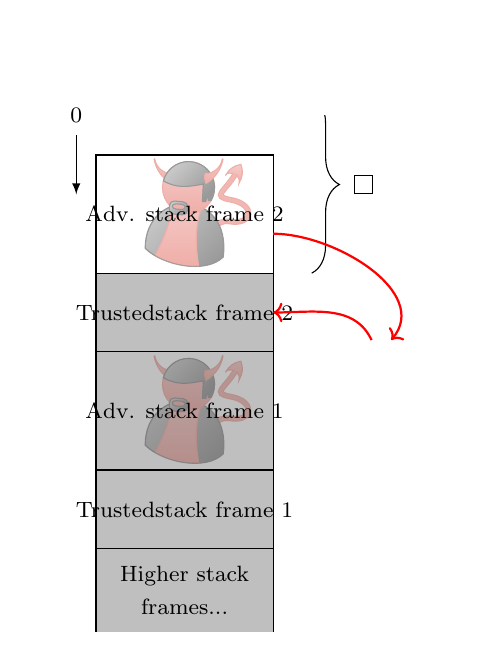
\begin{tikzpicture}[scale=.5, every node={scale=.5}]
      % recurrent parts
      \draw (-0.5,13) node {\footnotesize 0};
      \draw (-0.5,12.5) edge[thin,-latex] (-0.5,11);
      \stdstackstart[13]
      \inactsf{(0,2)}{(4.5,4)} {\footnotesize Trusted\\ \footnotesize stack frame 1}
      \inactadv{(0,4)}{(4.5,7)} {\footnotesize Adv. stack frame 1}
      \inactsf{(0,7)}{(4.5,9)} {\footnotesize Trusted \\ \footnotesize stack frame 2}
      \actadv{(0,9)}{(4.5,12)} {\footnotesize Adv. stack frame 2}

      % Stack pointer 1
      \begin{scope}
        \clip (4.6,4) rectangle (9,13);
        \capbracebot{(4.6,4)}{(4.6,13.5)}{adv. stack\\\footnotesize cap. 1}
      \end{scope}
      Stack pointer 2
      \begin{scope}
        \clip (4.8,4) rectangle (9,13);
        \capbrace{(5.2,9)}{(5.2,13.5)}{adv. stack\\\footnotesize cap. 2}
      \end{scope}

      \draw[red,thick,->] (4.5,10) to[out=0,in=50] node[midway,right] {} (7.5,7.3);
      \draw[red,thick,->] (7,7.3) to[out=115,in=0] node[midway,right] {} (4.5,8);
    \end{tikzpicture}
    \caption{An adversary uses a previous stack frame's stack pointer.}
    \label{fig:stack-ptr-abuse}
  \end{subfigure}
  \begin{subfigure}{0.18\linewidth}
    \phantom{testtestes}
  \end{subfigure}
  \begin{subfigure}{0.4\linewidth}
    \centering
    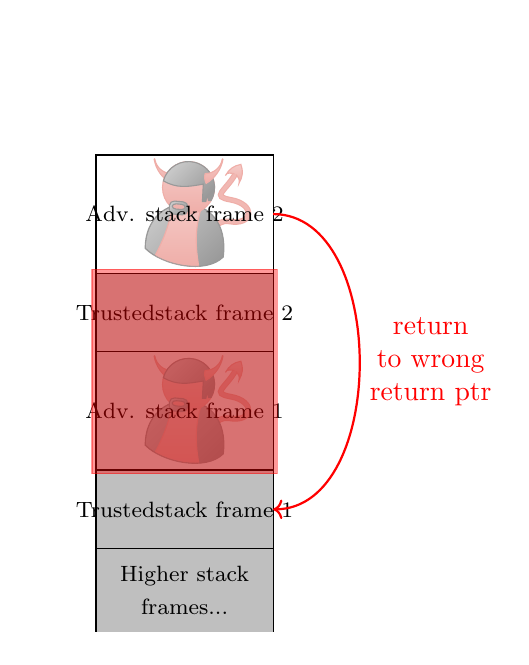
\begin{tikzpicture}[scale=.5, every node={scale=.5}]
      % recurrent parts
      \stdstackstart[13]
      \inactsf{(0,2)}{(4.5,4)} {\footnotesize Trusted\\ \footnotesize stack frame 1}
      \inactadv{(0,4)}{(4.5,7)} {\footnotesize Adv. stack frame 1}
      \inactsf{(0,7)}{(4.5,9)} {\footnotesize Trusted \\ \footnotesize stack frame 2}
      \actadv{(0,9)}{(4.5,12)} {\footnotesize Adv. stack frame 2}
      \fill[red,draw=red,opacity=.4] (-.1,3.9) rectangle (4.6,9.1);
      \draw[red,thick,->] (4.5,10.5) to[out=0,in=0] node[midway,right,align=center] {return\\ to wrong\\ return ptr} (4.5,3);
    \end{tikzpicture}
    \caption{An adversary jumps to a previous stack frame's stack pointer.}
    \label{fig:ret-ptr-abuse}
  \end{subfigure}
  
  \caption{Possible ways to abuse stack and return capabilities.}
  \label{fig:stack-ret-ptr-abuse}
\end{figure}

\stktokens{} is based on a traditional single stack, shared between all components.
As we are on a capability machine, it is natural to add some extra protection to stack and return pointers.
First, we replace stack pointers with stack capabilities.
When a new stack frame is created, the caller provisions it with a stack capability, restricted to the appropriate range, i.e.\ it does not cover the caller's stack frame.
Return pointers, on the other hand, are replaced by a pair of sealed return capabilities.
% KJAA: Again with the sealed pair. Again, this idea is unclear.
They form an opaque closure that the callee can only jump to, and the caller's data becomes available to the caller's return code. 

%informally explain how an adversary may try to abuse stack and return caps
While the above adds extra protection, it is not sufficient to enforce WBCF and LSE.
A callee that do not respect the calling convention (hence forward referred to as an adversary\footnote{The assumption on the adversary is described in detail in Section~\ref{sec:well-form-reas}.}) receives a stack capability and a return pair that they are supposed to use for the call, but the adversary can store the provided capabilities on the heap in order to use them later.
Figure~\ref{fig:stack-ret-ptr-abuse} illustrates two examples of this.
In both examples our component and an adversarial component have been taking turns calling each other, so the stack now contains four stack frames alternating between ours and theirs.
The figure on the left (Figure~\ref{fig:stack-ptr-abuse}) illustrates how we try to ensure LSE by restricting the stack capability to the unused part before every call to the adversary.
However, restricting the stack capability does not help when we, in the first call, give access to the part of the stack where our second stack frame will reside as nothing prevents the adversary from duplicating and storing the stack pointer.
Generally speaking, we have no reason to ever trust a stack capability received from an untrusted component as that stack capability may have been duplicated and stored for later use.
In the figure on the right (Figure~\ref{fig:ret-ptr-abuse}), we have given the adversary two pairs of sealed return capabilities, one in each of the two calls to the adversarial component.
The adversary stores the pair of sealed return capabilities from the first call in order to use it in the second call where they are not allowed.
The figure illustrates how the adversarial code uses the return pair from the first call to return from the second call and thus break WBCF.

% Informally explain how we prevent this using linear capabilities
As the examples illustrate, the standard memory and object-like capabilities (here sealed capabilities) do not seem to provide sufficient guarantees to enforce LSE and WBCF.
The problem is essentially that the stack and return pointers that a callee receives from a caller remain in effect after their intended lifetime: either when the callee has already returned or when they have themselves invoked other code. 
Linear capabilities offer a form of revocation\footnote{Revocation in the sense that if we hand out a linear capability and later get it back, then the receiver no longer has it or a copy of it as it is non-duplicable.} that can be used to prevent this from happening.

% Stack capability linear
The linear capabilities are put to use by requiring the stack capability to be linear.
On call, the caller splits the stack capability in two, such that they have a capability for their local stack frame and a capability for the unused part of the stack.
The stack capability for their local stack frame is sealed and used as the data part of the sealed return pair, and the stack capability for the remainder of the stack is given to the callee.
% Prevention of left attack non-aliasing of linear capabilities - token like (ensuring LSE)
Because the stack capability is linear, the caller knows that the capability for their local stack frame cannot have an alias.
This means that an adversary would need the stack capability produced by the caller in order to access their local data.
The caller gives this capability to the adversary only in a sealed form, rendering it opaque and unusable.
This is illustrated in Figure~\ref{fig:stack-ptr-abuse-prev} and prevents the issue illustrated in Figure~\ref{fig:stack-ptr-abuse}.

% Prevention of attack 2
In a traditional calling convention with a single stack, the stack serves as a call stack keeping track of the order calls where made in and thus in which order they should be returned to.
A caller pushes a stack frame to the stack on call and a callee pops a stack frame from the stack upon return.
However without any enforcement, there is nothing to prevent a callee from returning from an arbitrary call on the call stack.
This is exactly what the adversary does in Figure~\ref{fig:ret-ptr-abuse} when they skip two stack frames.
In the presence of adversarial code, we need some enforcement mechanism that allows us to make sure that the order of the call stack is kept.
One way to enforce this would be to hand out a token on call that can only be used when the caller's stack frame is on top of the call stack.
The callee would have to provide this token on return to prove that it is allowed to return to the caller, and on return the token would be taken back by the caller to prevent it from being spent multiple times.
As it turns out, the stack capability for the unused part of the stack can be used as such a token in the following way:
On return the callee has to give back the stack capability they were given on invocation.
When the caller receives a stack capability back on return, they need to check that this token is actually spendable, i.e.\ check whether their stack frame is on top of the call stack or not.
They do this by attempting to restore the stack capability from before the call by splicing the return token with the stack capability for the local stack frame which at this point has been unsealed again.
If the splice is successful, then the caller knows that the two capabilities are adjacent. On the other hand, if the splice fails, then they are alerted to the fact that their stack frame may not be the topmost.
\stktokens{} uses this approach; and as illustrated in Figure~\ref{fig:ret-ptr-abuse-prev}, it prevents the issue in Figure~\ref{fig:ret-ptr-abuse} as the adversary does not return a spendable token when they return.
\begin{figure}
  \centering
  \begin{subfigure}{0.4\linewidth}
    \centering
    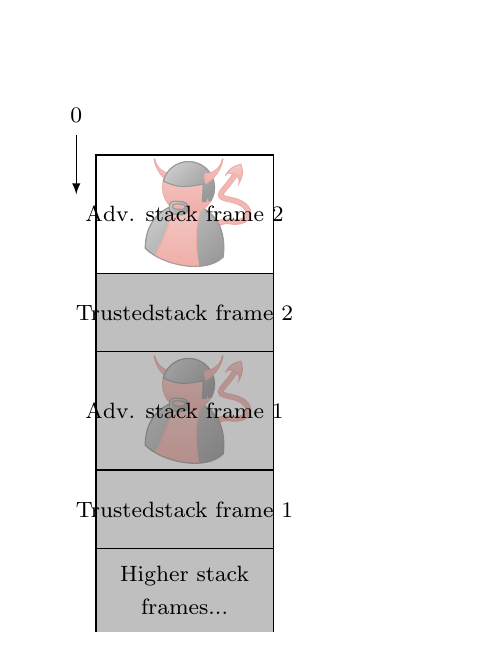
\begin{tikzpicture}[scale=.5, every node={scale=.5}]
      % recurrent parts
      \draw (-0.5,13) node {\footnotesize 0};
      \draw (-0.5,12.5) edge[thin,-latex] (-0.5,11);
      \stdstackstart[13]
      \inactsf{(0,2)}{(4.5,4)} {\footnotesize Trusted\\ \footnotesize stack frame 1}
      \inactadv{(0,4)}{(4.5,7)} {\footnotesize Adv. stack frame 1}
      \inactsf{(0,7)}{(4.5,9)} {\footnotesize Trusted \\ \footnotesize stack frame 2}
      \actadv{(0,9)}{(4.5,12)} {\footnotesize Adv. stack frame 2}

      \sealsymb{(4.9,3)}
      \lincapbrace{(4.6,2)}{(4.6,4)}{data return\\\footnotesize cap. 1}

      % Stack pointer 1
      \sealsymb{(4.9,5.5)}
      \lincapbrace{(4.6,4)}{(4.6,7)}{adv. stack\\\footnotesize cap. 1}
      % return cap
      \sealsymb{(4.9,8)}
      \lincapbrace{(4.6,7)}{(4.6,9)}{data return\\\footnotesize cap. 2}
     %  Stack pointer 2
      \begin{scope}
        \clip (4.8,4) rectangle (9,13);
        \lincapbrace{(4.6,9)}{(4.6,13.5)}{adv. stack\\\footnotesize cap. 2}
      \end{scope}

    \end{tikzpicture}
    \caption{The non-duplicable linear stack capability for the trusted code's
      stack frame and the opacity of sealed capabilities ensures LSE.}
    \label{fig:stack-ptr-abuse-prev}
  \end{subfigure}
  \begin{subfigure}{0.18\linewidth}
    \phantom{testtestes}
  \end{subfigure}
  \begin{subfigure}{0.4\linewidth}
    \centering
    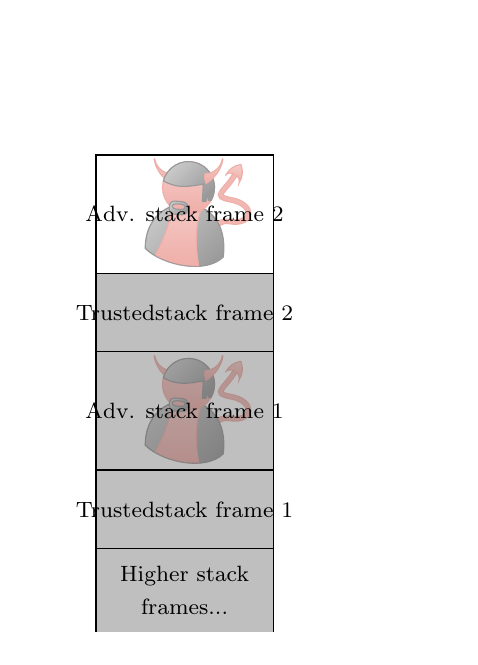
\begin{tikzpicture}[scale=.5, every node={scale=.5}]
      % recurrent parts
      \stdstackstart[13]
      \inactsf{(0,2)}{(4.5,4)} {\footnotesize Trusted\\ \footnotesize stack frame 1}
      \inactadv{(0,4)}{(4.5,7)} {\footnotesize Adv. stack frame 1}
      \inactsf{(0,7)}{(4.5,9)} {\footnotesize Trusted \\ \footnotesize stack frame 2}
      \actadv{(0,9)}{(4.5,12)} {\footnotesize Adv. stack frame 2}

      \lincapbrace{(4.6,2)}{(4.6,4)}{data return\\\footnotesize cap. 1}

     %  Stack pointer 2
      \begin{scope}
        \clip (4.8,4) rectangle (9,13);
        \lincapbrace{(4.6,9)}{(4.6,13.5)}{adv. stack\\\footnotesize cap. 2}
      \end{scope}

      \redcross{(5,4)}
    \end{tikzpicture}
    \caption{The trusted caller fails to splice the stack capability returned by
    the adversary with the capability for the trusted caller's local stack frame.}
    \label{fig:ret-ptr-abuse-prev}
  \end{subfigure}
  \caption{Abuse of stack and return capabilities prevention.}
\end{figure}

% Non-empty trusted stack frames.
In order for a call to have a presence on the call stack, its stack frame must be non-empty.
We cannot allow empty stack frames on the call stack, because then it would be impossible to tell whether the topmost non-empty stack frame has an empty stack frame on top of it.
Non-empty stack frames come naturally in traditional C-like calling convention as they keep track of old stack pointers and old program counters on the stack, but in \stktokens{} these things are part of the return pair which means that a caller with no local data may only need an empty stack frame.
This means that a caller using \stktokens{} needs to take care that their stack frame is non-empty in order to reserve their spot in the return order.
There is also a more practical reason for a \stktokens{} caller to make sure their stack frame is non-empty: They need a bit of the stack capability in order to perform the splice that verifies the validity of the return token.

% known stack base
% + more
At this point, the caller checks that the return token is adjacent to the stack capability for the caller's local stack frame and they have the means to do so.
However, this still does not ensure that the caller's stack frame is on top of the call stack.
The issue is that stack frames may not be tightly packed leaving space between stack frames in memory.
An adversarial callee may even intentionally leave a bit of space in memory above the caller's stack frame, so that they can later return out of order by returning the bit of the return token for the bit of memory left above the caller's stack frame.
This is illustrated in Figure~\ref{fig:stk-base-abuse}: In Figure~\ref{fig:stack-base-abuse-a}, a trusted caller has called an adversarial callee.
The adversary calls the trusted code back, but first they split the return token in two and store on the heap the part for the memory adjacent to the trusted caller's call frame (Figure~\ref{fig:stack-base-abuse-b}).
The trusted caller calls the adversary back using the precautions we have described so far (Figure~\ref{fig:stack-base-abuse-c}).
At this point (Figure~\ref{fig:stack-base-abuse-b}), the adversary has access to a partial return token adjacent to the trusted caller's first stack frame which allows the adversary to return from this call breaking WBCF.
For the caller to be sure that there are no hidden stack frames above its own, they need to make sure that the return token is exactly the same as the one they passed to the callee.
In \stktokens{}, the base address of the stack capability is fixed as a compile-time constant (Note: the stack grows downwards, so the base address of the stack capability is the top-most address of the stack). 
The caller verifies the validity of the return token by checking whether the base address of a returned token corresponds to this fixed base address, which was the base address for the return token they gave to the callee.
In the scenario we just sketched, the caller would be alerted to the attempt to break WBCF when the base address check of the return token fails in Figure~\ref{fig:stack-base-abuse-d}.

% Where do we get the stack pointer from, how can we know it is linear
% The other attack.
% At this point, the caller is able to verify whether a return token is spendable which allows them to decide whether they have the topmost stack frame on a call stack.
% However, in order to have WBCF there should only be one call stack, so the caller should also be able to verify that they have the top stack frame on the call stack used by all well-behaved components.
% In case a trusted component did not start the execution on the machine, i.e.\ they were called by another component, then the trusted component has no way to be sure whether the stack capability passed to them corresponds to the one and only call stack.
% To illustrate how an adversarial component can break WBCF by using multiple different stack capabilities consider this example: An adversary calls a trusted component with a callback and some linear capability that they claim is the stack capability.
% The trusted component executes using the stack capability given to them and at some point they invoke the callback, creating return tokens and so on.
% The adversary stores the return pair and return token and calls another trusted component but with a new callback and a new linear capability that they claim is the stack capability.
% Again, this trusted component also executes using the stack capability given to them and at some point they too invoke the callback, taking all the precautions we have described so far.
% At this point, the adversary has everything they need to return from either of the two callbacks.
% Specifically, they could return from the first callback invocation before they have returned from the second, breaking WBCF.
% From a high-level perspective, the problem is that both trusted components will be able to verify that they have the top stack frame on the call stack.
% They are both correct as the adversarial component has created two call stacks, one for each of the components.
% In order to solve this problem, the well-behaved code needs to somehow agree on the call stack.
% We do this by statically deciding on a global base address for the stack which is used for the entirety of the execution.
% A caller makes sure that they are using the correct stack by checking that the base address of the stack capability they receive corresponds to the global stack base address.
% This also means that on every return, the caller will check whether the return token's base address is equal to the global stack address.

In \stktokens{}, we ensure that at the start of execution the stack memory is only referenced by a single linear stack capability.
Because of this, we can assert validity of the return token simply by checking its base address and splicing it with the caller's stack frame.
There is no need to check linearity because we know that only linear capabilities to this memory exist.

% Return pointers/return seals
The return pointer in the \stktokens{} scheme is a pair of sealed capabilities where the code part of the pair is the old program counter, and the data part is the stack capability for the local stack frame of the caller.
Both of the capabilities in the pair are of course sealed with the same seal.
% One seal per return point
All call points need to be associated with a unique seal (a return seal) that is only used to seal the capabilities in the return pair for that particular call point.
The return seal is what associates the stack frame on the call stack with a specific call point in a program, so if we allowed return seals to be reused, it would be possible to return to a different call point than the one that caused the stack frame to be pushed on the call stack, which would break WBCF.
For similar reasons, we cannot allow return seals to be used to seal closures.
% Don't be stupid
Return seals should never be leaked to adversarial code as this would allow them to unseal the local stack frame of a caller breaking LSE.
This goes for direct leaks, such as leaving a seal in a register or writing it to adversarial memory, as well as indirect leaks, where a capability for reading a return seal (either directly or indirectly) from memory is leaked.

% Note about them vs us, we do nothing that they couldn't do
We have sometimes phrased the description of the \stktokens{} calling scheme in terms of ``them vs us''.
This may have created the impression of an asymmetric calling convention that places a special status on trusted components allowing them to protect themselves against adversaries.
However, \stktokens{} is a modular calling scheme: no restriction is put on adversarial components that we do not expect trusted components to meet.
Specifically, we are going to assume that both trusted and adversarial components are initially syntactically well-formed (described in more detail in Section~\ref{sec:well-form-reas}) which basically just restrict adversarial components to not break machine guarantees initially (e.g.\ no aliases for linear capabilities or access to seals of other components).
This means that any component can ensure WBCF and LSE by employing \stktokens{}.

% KJAA: ^-- Assuming that there is a global stack address capability, no?
Can I "suddenly" begin to impose \stktokens{}?

% Summary of CC
To summarise, our proposed calling convention \stktokens{} consists of the following measures:
\begin{enumerate}
\item \label{item:check-stkb} Check the base address of the stack capability before and after calls.
\item \label{item:non-empty-sf} Make sure that local stack frames are non-empty.
\item \label{item:return-data} Create token and data return capability on call: split the stack capability in two to get a stack capability for your local stack frame and a stack capability for the unused part of the stack. The former is sealed and used for the data part of the return pair.
\item \label{item:return-code} Create code return capability on call: Seal the old program pointer.
\item Reasonable use of seals: Return seals are only used to seal old program pointers, all return seals are only used for one call site, and they are not leaked.
\end{enumerate}
Item~\ref{item:check-stkb}-\ref{item:return-code} are captured by the code in Figure~\ref{fig:call-code} with the exception of checking stack base before calls. We do not include this check because it only needs to happen once between two calls which means that the check after a call suffices if the base of the stack pointer is not changed subsequently.

\begin{figure}
  \centering
  \begin{subfigure}{0.23\linewidth}
    \centering
    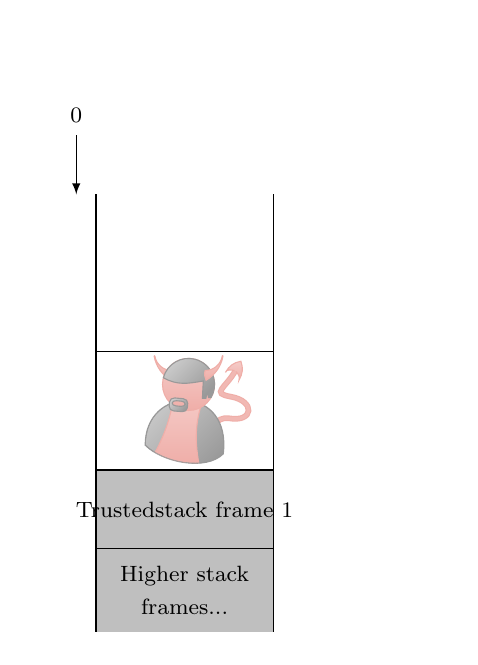
\begin{tikzpicture}[scale=.5, every node={scale=.5}]
      % recurrent parts
      \draw (-0.5,13) node {\footnotesize 0};
      \draw (-0.5,12.5) edge[thin,-latex] (-0.5,11);
      \stdstackstart[13]
      \inactsf{(0,2)}{(4.5,4)} {\footnotesize Trusted\\ \footnotesize stack frame 1}
      \actadv{(0,4)}{(4.5,7)}{}

      \sealsymb{(4.9,3)}
      \lincapbrace{(4.6,2)}{(4.6,4)}{}
      \begin{scope}
        \clip (4.8,1) rectangle (9,13);
      \lincapbracebot{(4.6,4)}{(4.6,13.5)}{}
      \end{scope}

    \end{tikzpicture}
    \caption{}
    \label{fig:stack-base-abuse-a}
  \end{subfigure}
  \begin{subfigure}{0.24\linewidth}
    \centering
    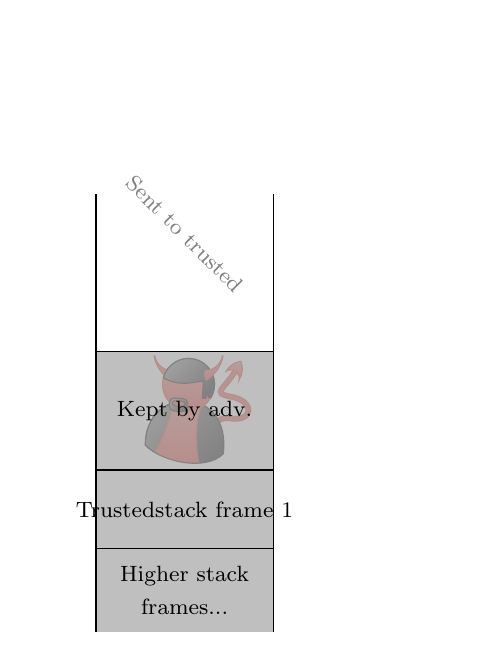
\begin{tikzpicture}[scale=.5, every node={scale=.5}]
      % recurrent parts
      \stdstackstart[13]
      \inactsf{(0,2)}{(4.5,4)} {\footnotesize Trusted\\ \footnotesize stack frame 1}
      \inactadv{(0,4)}{(4.5,7)}{\footnotesize Kept by adv.}
      \node[opacity=0.5,rotate=-45] at (2.25,10) {\footnotesize Sent to trusted};

      \sealsymb{(4.9,3)}
      \lincapbrace{(4.6,2)}{(4.6,4)}{}
      \lincapbrace{(4.6,4)}{(4.6,7)}{}
      
      \begin{scope}
        \clip (4.8,1) rectangle (9,13);
      \lincapbracebot{(4.6,7)}{(4.6,13.5)}{}
      \end{scope}

    \end{tikzpicture}
    \caption{}
    \label{fig:stack-base-abuse-b}
  \end{subfigure}
  \begin{subfigure}{0.24\linewidth}
    \centering
    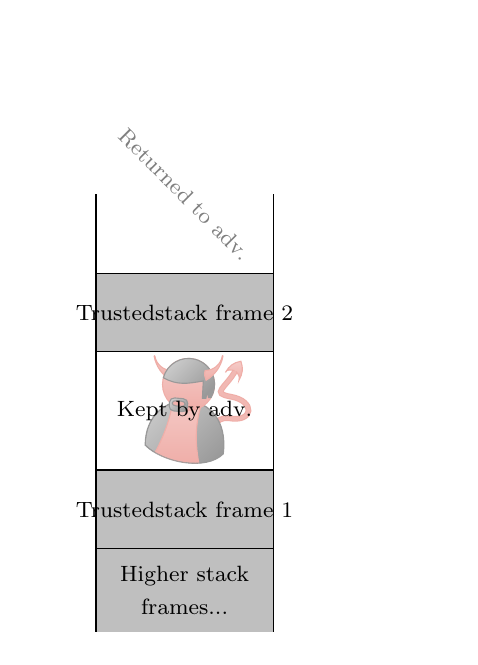
\begin{tikzpicture}[scale=.5, every node={scale=.5}]
      % recurrent parts
      \stdstackstart[13]
      \inactsf{(0,2)}{(4.5,4)} {\footnotesize Trusted\\ \footnotesize stack frame 1}
      \actadv{(0,4)}{(4.5,7)}{\footnotesize Kept by adv.}
      \inactsf{(0,7)}{(4.5,9)} {\footnotesize Trusted\\ \footnotesize stack frame 2}
      \node[opacity=0.5,rotate=-45] at (2.25,11) {\footnotesize Returned to adv.};
      \sealsymb{(4.9,3)}
      \lincapbrace{(4.6,2)}{(4.6,4)}{}
      \lincapbrace{(4.6,4)}{(4.6,7)}{}

      \sealsymb{(4.9,8)}
      \lincapbrace{(4.6,7)}{(4.6,9)}{}
      \begin{scope}
        \clip (4.8,1) rectangle (9,13);
        \lincapbracebot{(4.6,9)}{(4.6,13.5)}{}
      \end{scope}

    \end{tikzpicture}
    \caption{}
    \label{fig:stack-base-abuse-c}
  \end{subfigure}
  \begin{subfigure}{0.24\linewidth}
    \centering
    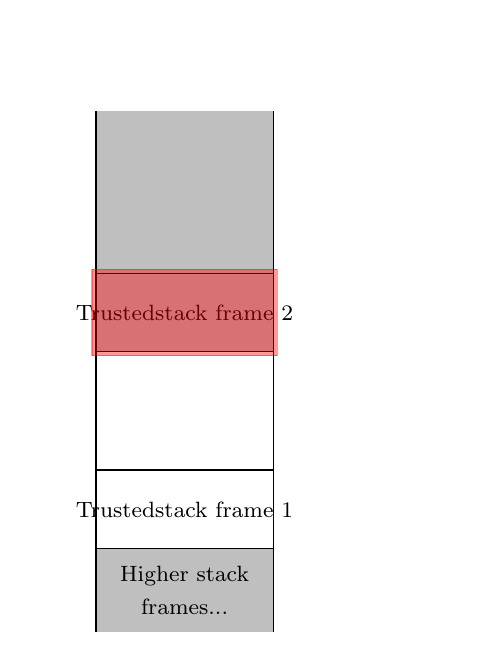
\begin{tikzpicture}[scale=.5, every node={scale=.5}]
      % recurrent parts
      \stdstackstart[13]
      \actsf{(0,2)}{(4.5,4)} {\footnotesize Trusted\\ \footnotesize stack frame 1}

      \inactsf{(0,7)}{(4.5,9)} {\footnotesize Trusted\\ \footnotesize stack frame 2}
      \begin{scope}
        \clip (-.1,-.1) rectangle (4.6,13.1);
        \draw[fill=gray!50] (0,9) rectangle (4.5,13.5);
      \end{scope}

      \lincapbrace{(4.6,2)}{(4.6,7)}{}

      \sealsymb{(4.9,8)}
      \lincapbrace{(4.6,7)}{(4.6,9)}{}

      \fill[red,draw=red,opacity=.4] (-.1,6.9) rectangle (4.6,9.1);
      \begin{scope}
        \clip (4.8,1) rectangle (9,13);
        \lincapbracebot{(4.6,9)}{(4.6,13.5)}{}
      \end{scope}

    \end{tikzpicture}
    \caption{}
    \label{fig:stack-base-abuse-d}
  \end{subfigure}
  \caption{Partial return token used to return out of order.}
  \label{fig:stk-base-abuse}
\end{figure}

\begin{figure}[htb]
  \centering
{\footnotesize
\[
  \begin{array}{r >{$}p{5.1cm}<{$} r l}
\multicolumn{2}{l}{\text{// Ensure non-empty stack.}}            & \multicolumn{2}{l}{\text{// Clear tmp registers and jump.}}\\
1 :& \tmove{\rtmp{1}}{42}                                        &14: & \tmove{\rtmp{1}}{0}\\
2 :& \tstore{\rstk}{\rtmp{1}}                                    &15: & \txjmp{r_1}{r_2}\\
3 :& \tcca{\rstk}{(-1)}                                          &\multicolumn{2}{l}{\text{// The following is the return code.}}\\
\multicolumn{2}{l}{\text{// Split stack in local stack frame and unused.}}      &\multicolumn{2}{l}{\text{// Check that returned stack pointer has base $\stkb$.}}\\
4 :& \tgeta{\rtmp{1}}{\rstk}                                     &16: & \tgetb{\rtmp{1}}{\rstk}\\
5 :& \tsplit{\rstk}{\rretd}{\rstk}{\rtmp{1}}                     &17: & \tminus{\rtmp{1}}{\rtmp{1}}{\stkb}\\
\multicolumn{2}{l}{\text{// Load the call seal.}}                &18: & \tmove{\rtmp{2}}{\pcreg}\\
6 :& \tmove{\rtmp{1}}{\pcreg}                                    &19: & \tcca{\rtmp{2}}{5}\\
7 :& \tcca{\rtmp{1}}{(\offpc - 5)}                               &20: & \tjnz{\rtmp{2}}{\rtmp{1}}\\
8 :& \tload{\rtmp{1}}{\rtmp{1}}                                  &21: & \rtmp{2}{1}\\
9 :& \tcca{\rtmp{1}}{\offsigma}                                  &22: & \tjmp{\rtmp{2}}\\
\multicolumn{2}{l}{\text{// Seal the local stack frame.}}        &23: & \tfail \\
10:& \tcseal{\rretd}{\rtmp{1}}                                   &\multicolumn{2}{l}{\text{// Splice with capability for local stack frame.}}\\
\multicolumn{2}{l}{\text{// Construct code return pointer.}}     &24: & \tsplice{\rstk}{\rstk}{\rdata} \\
11:& \tmove{\rretc}{\pcreg}                                      &\multicolumn{2}{l}{\text{// Pop 42 from the stack}}\\  
12:& \tcca{\rretc}{5}                                            &25: & \tcca{\rstk}{1}\\
13:& \tcseal{\rretc}{\rtmp{1}}                                   &\multicolumn{2}{l}{\text{// Clear tmp register}}\\
      &    &26: & \tmove{\rtmp{2}}{0}\\
  \end{array}
\]
}
\caption{
  % The instructions that constitutes a call. Register $r_1$ and $r_2$ are the registers where the sealed capability pair to the callee resides.
  % Variable $\offpc$ is the offset from the first instruction of the call to the set of seals, and $\offsigma$ is the offset to the seal within the set.
  % Instructions 1-3: ensure that the stack is non-empty.
  % Instructions 4-5: split stack pointer in two (stack pointer for callee done).
  % Instructions 6-9: Load the seal designated for this call.
  % Instruction 10: Seal capability for private stack to create data return pointer.
  % Instructions 11-13: Seal capability for return point to create code return pointer.
  % Instructions 14-15: Clean up temporary register and jump.
  % Instructions 16-26: The return code.
  % Instructions 16-23: check the stack base.
  % Instruction 24: join the stack pointer.
  % Instructions 25-26: pop 42 from the stack.
  The instructions for a $\scall{\offpc,\offsigma}{r_1}{r_2}$.
  The variable $\offpc$ is the offset from the first instruction of the call to the set of seals it uses.
  The variable $\offsigma$ is the offset in the set of seals to the call seal.
  The constant $\stkb$ is the globally agreed on stack base.
  There are a number of ``magic'' numbers in the code: line 1: $42$, garbage data to ensure a non-empty stack.
  Line 7: $-5$, offset to the first instruction of the call (from the point the capability was moved out of the $\pcreg$-register).
  Line 12: $5$, offset to the return address.
  Line 19: $5$, offset to fail.
  Line 21: offset to address after fail.
}
  \label{fig:call-code}
\end{figure}


% \begin{itemize}
% \item informally explain how an adversary may try to abuse stack and return caps
% \item informally explain how we prevent this using linear capabilities
% \item use the tikz pictures from the PriSC presentation to explain all of this
% \end{itemize}

\section{Formulating Security with a Fully Abstract Overlay Semantics}
\label{sec:form-secur-with}
As mentioned, the \stktokens{} calling convention guarantees well-bracketed control flow (WBCF) and local state encapsulation (LSE).
However, before we can prove these properties, we need to know how to even formulate them.
Although the properties are intuitively clear and sound precise, formalizing them is actually far from obvious.

Ideally, we would like to define the properties in a way that is
\begin{enumerate}
\item {\itshape intuitive} \label{def-prop:intuitive}
\item {\itshape useful for reasoning:} we should be able to use WBCF and LSE when reasoning about correctness and security of programs using \stktokens{}. \label{def-prop:useful}
\item {\itshape reusable in secure compiler chains:} for compilers using \stktokens{}, one should be able to rely on WBCF and LSE when reasoning about correctness and security of other compiler passes and then compose such results with our results to obtain results about the full compiler. \label{def-prop:reusable}
\item {\itshape arguably "complete"}: the formalization should arguably capture the entire meaning of WBCF and LSE and should arguably be applicable to any reasonable program. \label{def-prop:complete}
\item {\itshape potentially scalable}: even though we currently do not consider dynamic code generation or multi-threading, the current formalization should at least potentially extend to such settings. \label{def-prop:scalable}
\end{enumerate}

Previous formalisations in the literature are formulated in terms of a static control flow graph~\cite[e.g., ]{Abadi2005Theory}.
While these are intuitively appealing (\ref{def-prop:intuitive}), it is not clear how they can be used to reason about programs (\ref{def-prop:useful}) or other compiler passes (\ref{def-prop:reusable}), they lack temporal safety guarantees (\ref{def-prop:complete}) and do not scale (\ref{def-prop:scalable}) to settings with dynamic code generation (where a static control flow graph cannot be defined).
\citet{skorstengaard_reasoning_2017} provide a logical relation that can be used to reason about programs using their calling convention (\ref{def-prop:useful},\ref{def-prop:reusable}) it is not intuitive (\ref{def-prop:intuitive}), there is no argument for completeness (\ref{def-prop:complete}), and it is unclear whether it will scale to more complex features (\ref{def-prop:scalable}).

We contribute a new way to formalise the properties using a novel approach we call fully abstract overlay semantics.
The idea is to define a second operational semantics for programs in our target language.
This second semantics uses a different abstract machine and different run-time values, but it executes in lock-step with the original semantics and there is a very close correspondence between the state of both machines.

The main difference between the two semantics, is that the new one satisfies LSE and WBCF by construction: the abstract machine comes with a built-in stack, inactive stack frames are unaddressable and well-bracketed control flow is built-in to the abstract machine.
Important run-time values like return capabilities and stack pointers are represented by special syntactic tokens that interact with the abstract machine's stack, but during execution, there remains a close, structural correspondence to the actual regular capabilities that they represent.
For example, stack capabilities in the overlay semantics correspond directly to linear capabilities in the underlying semantics, and they have authority over the part of memory that the overlay views as the stack.

The fact that \stktokens{} enforces LSE and WBCF is formulated as a theorem about the function that maps components in the well-behaved overlay semantics to the underlying components in the regular semantics.
The theorem states that this function constitutes a fully abstract compiler, a well-known property from the field of secure compilation~\cite{abadi_protection_1999}.
Intuitively, the theorem states that if a trusted component interacts with (potentially malicious) components in the regular semantics, then these components have no more expressive power than components which the trusted component interacts with in the well-behaved overlay semantics.
In other words, they cannot do anything that doesn't correspond to something that a well-behaved component, respecting LSE and WBCF, can also do.
More formally, our full-abstraction result states that two trusted components are indistinguishable to arbitrary other components in the regular semantics iff they are indistinguishable to arbitrary other components in the overlay semantics.

Our formal results are complicated by the fact that they only hold for well-behaved components that respect the basic rules of the calling convention, and also on a sane initial configuration of the system.
For example, the system should be set up such that seals used by components for constructing return pointers are not shared with other components.
We envision distributing seals as a job for the linker, so this means our results depend on a linker to do this properly.
As another example, a seal used to construct a return pointer can be reused but only to construct return pointers for the same return point.
Different seals must be used for different return points.
Such seals should also never be passed to other components.
These requirements are easy to satisfy: components should request sufficient seals from the linker, use a different one for every place in the code where they make a call to another component, and make sure to clear them from registers before every call.
The general pattern is that $\stktokens{}$ only protects components that do not shoot themselves in the foot by violating a few basic rules.
In this section, we define a well-formedness judgement for the syntactic requirements on components as well as a reasonability condition that semantically disallows components to do certain unsafe things.

\begin{figure}[b]
  \centering
  \[
    \arraycolsep=1.4pt
    \begin{array}{rcl}
      \src{\SealableCaps} & \defbnf& \SealableCaps \mid \src{\stkptr{\permbnf,\basebnf,\aendbnf,\addrbnf}} \mid\\
                          & &   \src{\retptrd(\basebnf,\aendbnf)} \mid \src{\retptrc(\basebnf,\aendbnf,\addrbnf)}\\
      \multicolumn{3}{c}{
      \begin{array}{lcrclcr}
        \src{\StkFrame} & \defeq & \src{\Addr \times \MemSeg} & \phantom{skipskipsip} & \src{\Stack} & \defeq & \src{ \StkFrame^*}
      \end{array}
                                                                                                                }\\
      \src{\ExecConf} & \defeq & \Mem \times \Reg \; \src{\times \; \Stack \times \MemSeg} \\
    \end{array}
  \] 
\[
  \begin{array}{rcl}
    \offpc,\offsigma & \in & \nats \\
    \src{\Instr} & \defbnf &  \Instr \mid \scall{\offpc,\offsigma}{r}{r}
  \end{array}
\]
\caption{The syntax of \srccm{}.
  \srccm{} extends \trgcm{} by adding stack pointers, return pointers, and a built-in stack.
  Everything specific to the overlay semantics is written in blue.
}
  \label{fig:source-syntax}
\end{figure}

\todo[inline]{Dominique: I think it would be less confusing and more in line with the overlay semantics story to not add an extra instruction in Figure~\ref{fig:source-syntax} but rather present it as just a special case of the overlay semantics for the same underlying instructions.}

\subsection{Overlay semantics}
% Describe the things added to the syntax
The overlay semantics we define for \trgcm{} (\srccm{}) views part of the memory as a built-in stack (Figure~\ref{fig:source-syntax}).
% Built-in stack
To this end, it adds a call stack and a free stack memory to the executable configurations of \trgcm{}.
The call stack is a list with all the stack frames that are currently inaccessible because they belong to other calls.
A stack frame contains encapsulated stack memory as well as the program point execution is supposed to return to.
The free stack memory is the part of the stack that has not been claimed by a call and thus can be used at this point of time.
% Stack pointer
In order to distinguish capabilities for the stack from the capabilities for the rest of the memory, \srccm{} adds stack pointers.
A stack pointer has a permission, range of authority, and current address, just like capabilities on \trgcm{}, but they are always linear.
% Return pointers
The final syntactic constructs added by \srccm{} are the code and data return pointers.
The data return pointer corresponds to some stack pointer (which in turn corresponds to a linear capability), and the code return pointer corresponds to some capability with read-execute permission.
Syntactically, the return capabilities contain just enough information to reconstruct what they correspond to on the underlying machine.
On \srccm{}, return pointers are generated by calls from the capabilities they correspond to on \trgcm{}, and they are turned back to the capabilities they correspond to upon return.
% Even though the return pointers both correspond to capabilities with read permission, neither can be used for reading. 
% Say, we allowed reads through a data return pointer, then that would correspond to reading from some stack memory that is encapsulated in a stack frame which would break LSE.

The opaque nature of the return pointers is reflected in the interpretation of the instructions common to both \trgcm{} and \srccm{} as \srccm{} does not add special interpretation for them in non-\texttt{xjmp} instructions.
Stack pointers, on the other hand, need to behave just like capabilities, so \srccm{} adds new cases for them in the semantics, e.g.\ \texttt{cca} can now also change the current address of a stack pointer as displayed in Figure~\ref{fig:source-op-sem}.
Similarly, \texttt{load} and \texttt{store} work on the free part of the stack when provided with a stack pointer.
A store attempted with a stack capability that points to an address outside the free stack results in the $\failed$ configuration because that action is inconsistent with the view the overlay semantics has on the underlying machine.
In other words, there should only be stack pointers for the stack memory.

% Back to high-level view
As discussed earlier, our formal results only provide guarantees for components that respect the calling convention.
Untrusted components are not expected to take part in the calling convention.
To formalize this distinction, \srccm{} has a set of trusted addresses $\ta$.
Only instructions at these addresses can be interpreted as the \srccm{} native call and push frames to the call stack which guarantees LSE and WBCF.
The constant $\ta$ is a parameter of the \srccm{} step relation.
Similarly, \stktokens{} assumes a fixed base address of the stack memory, that is also passed around as such a parameter, for use in the native semantics of calls.

Apart from the step relation of \trgcm{}, \srccm{} has one overlay step that takes precedence over the others.
This step is shown in Figure~\ref{fig:source-op-sem}, and it is different from the others in the sense that it interprets a sequence of instructions rather than one.
The sequence of instructions have to correspond to a call, i.e.\ the
instructions in Figure~\ref{fig:call-code} ({\footnotesize  $\scall[i]{\offpc,\offsigma}{r_1}{r_2}$} corresponds to the $i$'th instruction in the figure and $\calllen$ is always $26$, i.e.\ the number of instructions).
Calls are only executed when the well-behaved component executes, so the addresses where the call resides must be in $\ta$, and the executing capability must have the authority to execute the call.

% Call/return
The interpretation of a call is also shown in Figure~\ref{fig:source-op-sem} and essentially does the following: It takes the local stack of the caller and puts it on the call stack along with the return address.
It also takes the stack capability for the local stack and a copy of the $\pc$-capability adjusted to point to the return address and turns them into a pair of sealed return capabilities.
The return capabilities are sealed with the seal designated for the call.

The return capabilities, $\retptrc$ and $\retptrd$, can only be used for returning.
Returns are handled by the \texttt{xjmp} instruction because the call produces sealed return capabilities.
Upon return, the topmost call stack frame $(\opc,\ms_\var{local})$ is popped from the call stack.
In order for the return to succeed, the return address in the code return pointer must match $\opc$, and the range of addresses in the data return pointer must be in the domain of the local stack.
If the return succeeds, then the stack pointer is reconstructed, and the local stack is moved back to be part of the active stack.

\srccm{} supports tail calls.
A tail call is a call from a caller that is done executing, and thus doesn't need to be returned to or preserve local state.
This means that a tail call should not reserve a slot in the return order by pushing a stack frame on the call stack, i.e.\ it should not use the built-in call.
To perform a tail call, the caller simply transfers control to the callee using \texttt{xjmp}.
The tail-callee should return to the caller's caller, so the caller leaves the return pair they received for the callee to use.

It is important to observe that the operational semantics of \srccm{} natively guarantee WBCF (well-bracketed control flow) and (local stack encapsulation) for calls made by trusted components.
By inspecting the operational semantics of \srccm{}, we can see that it never allow reads or writes to inactive stack frames on the call stack.
The built-in call for trusted code pushes the local stack frame to the inactive part of the stack, together with the return address. 
Such frames can be reactivated by \texttt{xjmp}ing to a return capability pair, but only for the topmost stack frame and if the return address corresponds to the one stored in the call stack.
In other words, WBCF and LSE are natively enforced in this semantics.

\begin{figure}[htb]
  \centering
  \begin{mathpar}
    \inferrule{\src{\Phi(\pcreg) = ((\perm,\_),\baddr,\eaddr,\aaddr)} \\
               \src{\lbrack \aaddr ,\aaddr + \calllen - 1\rbrack \subseteq \ta}  \\
               \src{\lbrack\aaddr,\aaddr + \calllen-1\rbrack \subseteq [\baddr,\eaddr]} \\
               \src{\perm \in \{\rwx,\rx\}} \\
               \src{\Phi.\mem(\aaddr,\dots,\addr + \calllen-1) = \scall[0]{\offpc,\offsigma}{r_1}{r_2} \cdots \scall[\calllen-1]{\offpc,\offsigma}{r_1}{r_2}}
 }
              { \src{\Phi}  \; \src{\step[\src{\ta,\stkb}] \sem{\scall{\offpc,\offsigma}{r_1}{r_2}}(\Phi)} }
  \end{mathpar}
  \begin{tabular}{|>{$}c<{$}|p{3.7cm}|>{\raggedright\arraybackslash}p{6.6cm}|}
    \hline
    i \in \src{\Instr}                                 & $\sem{i}(\Phi)$ & Conditions\\
    \hline
    \halt                                        & $\halted$ & \\
    \hline
    \multicolumn{3}{|c|}{\dots\text{ (the operational semantics of \trgcm)}} \\
    \hline
    \store{r_1}{r_2}                             & $\srcalt{\var{updPc}} \sourcecolor\arraycolsep=0pt\array[t]{rl}(\Phi&\updReg{r_2}{w_2}\\ &\update{\ms_\stk.\aaddr}{\Phi(r_2)})\endarray$  & \srcalt{$\Phi(r_1) = \stkptr{\perm,\baddr,\eaddr,\aaddr}$ and $\perm \in \{\rwx,\rw\}$ and $\baddr \le \aaddr \le \eaddr$ and $w_2 = \linCons{\Phi(r_2)}$ and $\aaddr \in \dom(\ms_\stk)$}\\
    \hline
    \cca{r}{\rn}                                 &$\srcalt{\updPcAddr{\Phi\updReg{r}{w}}}$ &  \srcalt{$\Phi(\rn) = n \in \ints$ and $\Phi(r) = \stkptr{\perm,\baddr,\eaddr,\aaddr}$ and $w = \stkptr{\perm,\baddr,\eaddr,\aaddr+n}$} \\
    \hline
    \arraycolsep=0pt\array{c}
    \scall{\srcalt{\offpc,\offsigma}}{\src{r_1}}{\src{r_2}}
    \endarray &
        $\srcalt{\var{xjmpRes}(c_1,c_2,}$
        $\srcalt{\hspace{.25cm}\left(\arraycolsep=0pt\array[c]{rl}\Phi&\updReg{r_1,r_2}{w_1,w_2}\\
            &\updReg{\rretc}{s_c}\\
            &\updReg{\rretd}{s_d}\\
            &\updReg{\rstk}{c_\stk}\\
            &\update{\ms_\stk}{\ms_{\stk,\var{rest}}}\\
            &\update{\stk}{\stk'}\\
            \endarray\right))}$
       &
      \srcalt{$\stk' = (\opc,\ms_{\stk,\var{local}}) :: \Phi.\stk$ and 
         $\begin{multlined}
           \ms_{\stk,\var{local}},c_\var{local},\ms_{\stk,\var{rest}},c_\stk =\\ \var{splitStack}(\Phi.\reg(\rstk), \Phi.\ms_\stk) \text{ and }
         \end{multlined}$
    $\opc, c_\opc =\var{setupOpc(\Phi.\reg(\pcreg))}$ and
    $\sigma =\begin{multlined}[t]
      \var{getCallSeal}(\\
      \Phi.\reg(\pcreg), \Phi.\mem,\offpc,\offsigma)  \text{ and }
    \end{multlined}$
    $s_c,s_d = \var{sealReturnPair}(\sigma,c_\opc,c_\var{local})$ and
    $w_1,w_2 = \linCons{\Phi.\reg(r_1,r_2)}$ and
                        $\Phi.\reg(r_1,r_2) = \sealed{\sigma', c_1}, \sealed{\sigma', c_2}$
                        }\\
    \hline 
    \multicolumn{3}{|c|}{\dots} \\
    \hline
    \_                                           & $\failed$ & \totherwise \\
    \hline
  \end{tabular}
\begin{multline*}
  \srcxjmpres{c_1,c_2,\Phi} = \\
  \left\{ 
    \arraycolsep=1.4pt
    \begin{array}{l c >{\raggedright\arraybackslash}p{9.5cm}}
      \arraycolsep=0pt
    \begin{array}{rl}
      \Phi & \updReg{\pcreg}{c_1}\\
           & \updReg{\rdata}{c_2}
    \end{array}
    &\phantom{mak} & $\nonExec{c_2}$ \srcalt{and $c_1 \neq \retptrc(\_)$ and $c_2 \neq \retptrd(\_)$}\\
      \arraycolsep=0pt
      \array[c]{rl}
      \Phi&\updReg{\pcreg}{c_\opc}\\
          &\updReg{\rstk}{c_\stk}\\
          &\updReg{\rdata}{0}\\
          &\update{\stk}{\stk'}\\
          &\update{\ms_\stk}{\ms_\stk \uplus \ms_\var{local}}
      \endarray
           & &
               $\arraycolsep=0pt\array{l}
        \src{(\opc, \ms_\var{local}) :: \stk'= \Phi.\stk \tand} \\
      \src{c_1 = \retptrc(\baddr,\eaddr,\opc)}\\
      \src{c_2 = \retptrd(\aaddr_\stk,\eaddr_\stk) \wedge \dom(\ms_\var{local}) = [\aaddr_\stk,\eaddr_\stk]}\\
      \src{c_\stk = \var{reconstructStackPointer}(\reg(\rstk),c_2) \tand}\\
      \src{c_\opc =  ((\rx,\normal),\baddr,\eaddr,\opc)} 
      \endarray$\\
      \failed &  & \totherwise
    \end{array} 
\right.
\end{multline*}
  \caption{An excerpt of the operational semantics of \srccm{} (some details omitted). Auxiliary definitions are found in Figure~\ref{fig:source-op-sem-aux}. }
  \label{fig:source-op-sem}
\end{figure}


\begin{figure}
    \begin{multline*}
      \src{\var{splitStack}(\stkptr{\rw,\baddr_\stk,\eaddr_\stk,\aaddr_\stk}, \ms_\stk) = \ms_{\stk,\var{local}},c_\var{local\_data},\ms_{\stk,\var{unused}},c_\stk} \mathit{\ iff\ } \\
      \left\{ 
      \begin{array}{l}
      \src{\baddr_\stk < \aaddr_\stk \leq \eaddr_\stk }\\
      \src{\ms_{\stk,\var{local}} = \ms_\stk |_{[\aaddr_\stk,\eaddr_\stk]}\update{\aaddr_\stk}{42} }\\
      \src{\ms_{\stk,\var{unused}} = \ms_\stk|_{[\baddr_\stk,\aaddr_\stk-1]} }\\
      \src{c_\stk = \stkptr{\rw,\baddr_\stk,\aaddr_\stk-1,\aaddr_\stk-1} }\\
      \src{c_\var{local\_data} = \retptrd(\aaddr_\stk,\eaddr_\stk) }\\
      \end{array}
      \right.
    \end{multline*}
    \begin{align*}
      \src{ \var{setupOpc(((\_,\_),\baddr,\eaddr,\aaddr))}} &\ \src{= \opc, c_\opc} \mathit{\ iff\ }
      \left\{ 
      \begin{array}{l}
      \src{\opc = \aaddr + \calllen \wedge{}}\\
      \src{c_\opc = \retptrc(\baddr,\eaddr,\opc) \wedge{}}
      \end{array}
       \right.\\
      \src{\var{getCallSeal}(c_\pcreg,\mem,\offpc,\offsigma)} &\ \src{= \sigma} \mathit{\ iff\ }
      \left\{
      \begin{array}{l} 
      \src{c_\pcreg = ((\_,\_),\baddr,\eaddr,\aaddr) \wedge \baddr \leq  \aaddr+\offpc \leq \eaddr \wedge{}} \\
      \src{\mem(\aaddr+\offpc) = \seal{\sigma_\baddr,\sigma_\eaddr,\sigma_\aaddr} \wedge{} \sigma_\baddr \leq \sigma \leq \sigma_\eaddr \wedge{}}\\
      \src{\sigma = \sigma_\aaddr + \offsigma }
      \end{array}
      \right.\\
     \src{\var{sealReturnPair}(\sigma,c_\opc,c_\var{local})} &\ \src{= \sealed{\sigma,c_\opc},\sealed{\sigma,c_\var{local}}}
    \end{align*}%
  % \begin{multline*}
  %   \src{\var{callConditions}(r_1,r_2,\offpc,\offsigma,(\mem,\reg,\stk,\ms_\stk)) = (\mem,\reg',\stk',\ms_{\stk,\var{rest}})}\mathit{\ iff}\\
  %     \quad\quad\left\{ 
  %       \begin{array}{l}
  %         \src{\var{sealedPairArgument}(\reg,r_1,r_2,c_1,c_2)}\\
  %     \src{\ms_{\stk,\var{local}},\ms_{\stk,\var{rest}},c_\stk,c_\var{local\_data} = \var{splitStack}(\reg, \ms_\stk) \wedge{}}\\
  %     \src{\opc, c_\opc =\var{setupOpc(\reg)} \wedge{}}\\
  %     \src{\stk' = (\opc,\ms_{\stk,\var{local}}) :: \stk \wedge{}}\\
  %     \src{\sigma = \var{getCallSeal}(\reg,\mem,\offpc,\offsigma) \wedge{}}\\
  %     \src{s_c,s_d = \var{sealReturnPair}(\sigma,c_\var{local\_data},c_\opc) \wedge{}}\\
  %     \src{w_1,w_2 = \linCons{\reg(r_1),\reg(r_2)} \wedge{}}\\ 
  %     \src{\reg' =\reg\updReg{r_1,r_2}{w_1,w_2}\updReg{\rretc,\rretd}{s_c,s_d}\updReg{\rstk,\rtmp{1}}{c_\stk,0}}
  %     \end{array}\right.
  % \end{multline*}
  \begin{multline*}
    \src{\var{reconstructStackPointer}(\stkptr{\rw, \stkb, \aaddr_\stk-1,\_},\retptrd(\aaddr_\stk,\eaddr_\stk)) =}\\ \src{\stkptr{\rw,\stkb,\eaddr_\stk,\aaddr_\stk}} \mathit{\ iff\ }
        \src{\stkb \leq \addr_\stk }
   \end{multline*}

  \caption{Auxiliary definitions used in the operational semantics of \srccm{}.}
  \label{fig:source-op-sem-aux}
\end{figure}
% \begin{figure}
% % \[
% %     \src{\stkptr{\rw,\stkb,\eaddr_\stk,\aaddr_\stk} = \var{tokenToStkPtr}(\retptrd(\aaddr_\stk,\eaddr_\stk)}
% % \]
% % \[
% %     \src{\stk', \ms_\var{local\_stk} = \var{popCallStackFrame} (\stk,c_1,c_2)}
% %     \mathit{\ iff\ }
% %       \left\{ \array{l}
% %         \src{\stk = (\opc, \ms_\var{local\_stk}) :: \stk' \wedge{}} \\
% %         \src{c_1 = \retptrc(\_,\_,\opc) \wedge{}} \\
% %         \src{c_2 = \retptrd(\aaddr_\stk,\eaddr_\stk)\wedge{}} \\
% %         \src{\dom(\ms_\var{local\_stk}) \subseteq [\aaddr_\stk,\eaddr_\stk]}
% %         \endarray
% %      \right.
% % \]
% % \[
% %   \src{\var{retPtrForMatchLocalStack(\retptrd(\aaddr_\stk,\eaddr_\stk),\ms_\var{local})}} \mathit{\ iff\ } \src{\dom(\ms_\var{local} \subseteq [\aaddr_\stk,\eaddr_\stk])}
% % \]

% % \begin{multline*}
% %     \src{(\mem,\reg',\stk',\ms_\stk') = \var{returnCondition}(c_1,c_2,(\mem,\reg,\stk,\ms_\stk))}\mathit{\ iff\ }\\
% %       \quad\quad\left\{ 
% %       \begin{array}{l}
% %       \src{\stk', \ms_\var{local\_stk} = \var{popCallStackFrame}(\stk,c_1,c_2)}\\
% %       \src{c_\stk = \var{reconstructStackPointer}(\reg,c_2)}\\
% %       \src{c_\opc =  \var{tokenToPc}(c_1)} \\
% %       \src{\ms_\stk' = \ms_\stk \uplus \ms_\var{local\_stk}} \\
% %       \src{\reg' =\reg\updReg{\pcreg,\rstk}{c_\opc,c_\stk}\updReg{\rdata,\rtmp{1},\rtmp{2}}{0,0,0}}
% %       \end{array}\right.
% %   \end{multline*}

%   \caption{The return condition in the operational semantics of \srccm{}.}
%   \label{fig:source-op-sem-return}
% \end{figure}
\subsection{Well-formedness and reasonability}
\label{sec:well-form-reas}
% Well-formed components
% \begin{figure}[htb]
%   \centering
%   \begin{mathpar}
%   \inference{
%     \dom(\mscode) = [\baddr,\eaddr]&
%     [\baddr-1,\eaddr+1] \mathrel{\#} \dom(\msdata)\\
%     \mspad = [\baddr-1\mapsto 0] \uplus [\eaddr+1 \mapsto 0]\\
%     \sigrets,\sigcloss \vdash_{\mathrm{comp-code}} \mscode \\
%     \exists A_\mathrm{own} : \dom(\msdata) \rightarrow \powerset{\dom(\msdata)} & \dom(\msdata) = A_{\mathrm{non-linear}} \uplus A_\linear \\
%     A_\linear = \biguplus_{a \in \dom(\msdata)} A_{\mathrm{own}}(a) \\
%     \forall a \in \dom(\msdata)\ldotp \dom(\mscode),A_{\mathrm{own}}(a),A_{\mathrm{non-linear}},\sigrets,\sigcloss \vdash_{\mathrm{comp-value}} \msdata(a)\\
%     \overline{\var{export}} = \overline{s_{\mathrm{export}} \mapsto w_{\mathrm{export}}} & \overline{\var{import}} = \overline{a_{\mathrm{import}} \mapsfrom s_{\mathrm{import}}}& \{\overline{a_{\mathrm{import}}}\} \subseteq \dom(\msdata)\\
%     \overline{\dom(\mscode), A_{\mathrm{non-linear}}, \sigrets,\sigcloss \vdash_{\mathrm{comp-export}} w_{\mathrm{export}}}\\
%     \overline{s_{\mathrm{import}}} \mathrel{\#} \overline{s_{\mathrm{export}}} & (\dom(\mscode) \subseteq \ta) \vee (\dom(\mscode) \mathrel{\#} \ta \wedge \sigrets = \emptyset)&
%     \dom(\msdata) \mathrel{\#} \ta
%   }{
%     \vdash (\mscode\uplus \mspad,\msdata,\overline{\var{import}},\overline{\var{export}},\sigrets,\sigcloss,A_\linear)
%   }
%   \and
%   \inference{
%     \comp_0 = (\mscode,\msdata,\overline{\var{import}},\overline{\var{export}},\sigrets,\sigcloss,A_\linear)\\
%     \vdash \comp_0 & (\_ \mapsto c_{\mathrm{main},c}), (\_ \mapsto c_{\mathrm{main},d}) \in \overline{\var{export}}
%   }{
%     \vdash (\comp_0,c_{\mathrm{main},c}, c_{\mathrm{main},d})
%   }
% \end{mathpar}
%   \caption{Exceprt of well-formedness judgement}
%   \label{fig:well-formedness}
% \end{figure}
% Well-formedness highlights:
% Main exported
% Code memory:
% - Only instructions and seals
% - calls associated with return seals unique return seal
% - only uses seals specified for components
% - (No linear access)
% Data memory:
% - Data
% - Capabilities fora data memory (linearity respected)
% - Sealed caps sealed with clos seal
% Exports
% - Any Word valid in data memory or
% - Sealed capability for code (sealed with clos seal)
% Imports
% - Address must be in data memory
The judgement $\wdjud[\ta]{\comp}$ specifies what components are well formed, i.e.\ satisfy the initial syntactic requirements necessary to be able to rely on system guarantees.
We elide the details of the judgement here and describe the main points:
For components with a main pair, the main pair must come from the exports and the remainder of the component must be well-formed.
As a reminder, a base component looks like this: $(\mscode,\msdata,\overline{\var{import}},\overline{\var{export}},\sigrets,\sigcloss,A_\linear)$.
The return seals $\sigrets$ are the seals supposed to be used to seal return pointers and the closure seals $\sigcloss$ all the other seals in a component .
If a component is adversarial, i.e.\ the domain of the code memory $\mscode$ is disjointed from the set of trusted addresses $\ta$, then there should be no return seals.
The code memory may contain sets of seals but only the seals in $\sigrets$ and $\sigcloss$.
Other than that, code memory only contains instructions in the form of integers.
When a sequence of instructions in the code memory corresponds to a call (Figure~\ref{fig:call-code}), the call must have access to the return seal it specifies.
The return seal also needs to be unique to that call; that is, no other call can specify the same seal as its return seal.
The data memory $\msdata$ may contain data, capabilities, and sealed capabilities.
The capabilities in the data memory can only have authority over the data memory itself.
This allows components to have initial data structures.
In order to respect Write-XOR-Execute, the capabilities in data memory cannot have execute permission.
The capabilities also need to respect linearity which means that linear capabilities cannot be aliased by any other capability, and they must be for a range of the predetermined linear addresses $A_\linear$.
The sealed capabilities must be sealed with a closure seal, and the sealable can be anything that is allowed to reside in data memory.
The exports $\overline{\var{export}}$ can be anything non-linear allowed to reside in data memory or a sealed capability for the code memory sealed with one of the closure seals.

% Reasonability
The static guarantees given by $\wdjud[\ta]{\comp}$ makes sure that components initially don't undermine the security measures needed for \stktokens{}, but it does not prevent a component from doing something silly during execution that undermines \stktokens{}.
In order for \stktokens{} to provide guarantees for a component, we expect it to not shoot itself in the foot and perform certain necessary checks not captured by the call code (Figure~\ref{fig:call-code}).
More precisely, we expect four things of a reasonable component: (1) It checks the stack base address before performing a call.
As explained in Section~\ref{sec:stktokens-explained}, we do not include this check in the call code as it often would be redundant.
(2) It uses the return seals only for calls and the closure seals in an appropriate way which means that they should only be used to seal executable capabilities for code that behaves reasonably or non-executable things that do not undermine the security mechanisms \stktokens{} relies on.
(3) It does not leak return and closure seals or means to retrieve them.
This means that sets of seals with return or closure seals cannot be left in registers when transferring control to another module.
There are also indirect ways to leak seals such as leaking a capability for code memory or leaking a capability for code memory sealed with an unknown seal.
(4) It does not store return and closure seals or means to get them.
By disallowing this, we make sure that data memory always can be safely shared as it does not contain seals or means to get them to begin with.
We elide the details here and refer to~\citet{technical_report}

In our result, we assume that adversarial components are well-formed, but not necessarily reasonable. The well-formedness assumption ensures that the trusted component can rely on basic security guarantees provided by the capability machine. For instance, if we did not require linearity to be respected initially, then adversarial code could start with an alias for the stack capability. The adversary is not assumed to be reasonable as we do not expect them to obey the calling convention in any way. Can adversarial code call into trusted components? The answer to that question is yes but not with LSE and WBCF guaranteed. Formally, adversarial code can contain the instructions that constitute a call. However, for untrusted code, \srccm{} will not execute those instructions as a "native call" but execute the individual instructions separately. The callee then executes in the same stack frame as the caller, so WBCF and LSE do not follow (for that call).

We will assume trusted component, for which WBCF and LSE are guaranteed, to be both well-formed and reasonable. 
%The reasonability definition has also been left out for space reasons, and we refer to the technical report~\citep{technical_report} for full definitions.

% \begin{definition}[Reasonable configuration]
%   \label{def:reasonable-conf}
%   We say that an execution configuration $\Phi$ is reasonable up to $n$ steps with $(\ta,\stkb,\gsigrets,\gsigcloss)$ 
%   iff for $n' \leq n$:
%   \begin{itemize}
%   \item \emph{Guarantee stack base address before call...}
%   \item \emph{Use return seals only for calls, use closure seals appropriately...}
%   \item \emph{Don't store private stuff...} If $\src{\Phi}$ points to $\src{\tstore{r_1}{r_2}}$ in $\ta$, then

%     Then $n' = 0$ or $\Phi.\reg(r_2)$ is reasonable in memory $\Phi.\mem$ up to $n' -1$ steps.
%   \item \emph{Don't leak private stuff...}
%   \end{itemize}
% \end{definition}
% Reasonable configuration
% Reasonable component


\subsection{Full abstraction}
All that is left before we state the full-abstraction theorem is to define how components are combined with contexts and executed, so that we can define contextual equivalence.

% How a program is lifted to an executable configuration
Given a program $\var{comp}$, the judgement $\var{comp} \rightsquigarrow \Phi$ defines an initial execution configuration that can be executed.
It works almost the same on \trgcm{} and \srccm{}.
On both machines a stack containing all zeroes is added, as part of the regular memory on \trgcm{} and as the free stack on \srccm{}.
On \srccm{}, the initial stack is empty as no calls have been made.
The component needs access to the stack, so a stack pointer is added to the register file in $\rstk$.
On \trgcm{} this is just a linear read-write capability, but on \srccm{} it is the representation of a stack pointer.
The entry point of the program is specified by main, so the two capabilities are unsealed (they must have the same seal) and placed in the $\pcreg$ and $\rdata$ registers.
Other registers are set to zero.

Contextual equivalence roughly says that two components behave the same no matter what context we plug them into.
%The remaining defintions
\begin{definition}[Plugging a component into a context]
  \label{def:comp-context-plugging}
  When $\var{comp'}$ is a context for component $\var{comp}$ and $\var{comp}' \bowtie \var{comp} \rightsquigarrow \Phi$, 
  then we write $\plug{\var{comp'}}{\var{comp}}$ for the execution configuration $\Phi$.
\end{definition}
\begin{definition}[\trgcm{} and \srccm{} contextual equivalence]
  \label{def:contextual-equivalence}
  ~
  \begin{description}
  \item[On \srccm{}], we define that $\src{\comp_1 \sconeq \comp_2}$ iff
  \begin{equation*}
    \forall \src{\context} \ldotp  \wdjud[\emptyset]{\src{\context}} \Rightarrow \src{\plug{\context}{\comp_1} \sterm{\ta[,1],\stkb_1}} \Leftrightarrow \src{\plug{\context}{\comp_2} \sterm{\ta[,2],\stkb_2}}
  \end{equation*}
  with $\src{\ta[,i]} = \src{\dom(\comp_i.\mscode)}$.
  \item[On \trgcm{}], we define that $\trg{\comp_1 \tconeq \comp_2}$ iff
  \begin{equation*}
    \forall \trg{\context} \ldotp \wdjud[\emptyset]{\trg{\context}} \Rightarrow \trg{\plug{\context}{\comp_1} \term} \Leftrightarrow \trg{\plug{\context}{\comp_2} \term}
  \end{equation*}
\end{description}
where $\Phi\sterm[i]{\src{\ta,\stkb}} \text{ iff } \Phi \nstep[i]{\src{\ta,\stkb}} \halted \quad$ and $\quad \Phi\sterm{\src{\ta,\stkb}} \defeq \exists i \ldotp \sterm[i]{\src{\ta,\stkb}}$
\end{definition}
With the above defined, we are almost ready to state our full-abstraction, and all that remains is the compiler we claim to be fully-abstract.
We only care about the well-formed components, and they sport none of the new syntactic constructs \srccm{} adds to \trgcm{}.
This means that the compilation from \srccm{} components to \trgcm{} components is simply the identity function.
% Full abstraction thm
\todo[inline]{Look at coloring in these theorems. Why are all components and contexts blue?}
\begin{theorem}
  \label{thm:full-abstraction}
  For reasonable, well-formed components $\comp_1$ and $\comp_2$, we have
  \begin{gather*}
    \src{\comp_1} \sconeq \src{\comp_2} \quad \Leftrightarrow \quad    \src{\comp_1} \tconeq \src{\comp_2} \qedhere
  \end{gather*}
\end{theorem}
Readers unfamiliar with fully-abstract compilation may wonder why Theorem~\ref{thm:full-abstraction} proves that \stktokens{} guarantees LSE and WBCF.
Generally speaking, behavioral equivalences are preserved and reflected by fully-abstract compilers.
This means that any property the source language has must somehow be there after compilation whether or not it is a property of the target language.
If the source language has a property that the target language doesn't have, then a compiled source program must use the available target language features to emulate the source language property in a way that it behaviorally matches exactly.
In our case, LSE and WBCF was built into the semantics of \srccm{}, but they are not properties of \trgcm{}.
In order to enforce these properties, components on \trgcm{} use \stktokens{}.
Theorem~\ref{thm:full-abstraction} proves that \stktokens{} enforces these properties in a way that behaviorally matches \srccm{} which means that it enforces LSE and WBCF.
\todo[inline]{Consider writing a bit more about compiler correctness and contextual equivalence preservation.}



% \begin{itemize}
% \item present our source language, its operational semantics (excerpts)
% \item tell more about components, specifically well-formed according to judgement
% \item mention our assumption of reasonability
% \item present the full abstraction theorem.
% \end{itemize}

\section{Proving full abstraction}
\label{sec:fa-proof}
%\todo[inline]{Write small introduction. Maybe something about the difficulty of full-abstraction proofs (with references?) but mention that this is easier than some other cases (reference approximate back translation?) because back translation is trivial.}
% \begin{itemize}
% \item Logical relation
% \item FTLR
% \item Sketch high-level structure of the proof
% \end{itemize}
To prove Theorem~\ref{thm:full-abstraction}, we will essentially show that trusted components in \srccm{} are related in a certain way to their embeddings in \trgcm{}, and that untrusted \trgcm{} components are similarly related to their embeddings in \srccm{}.
We will then prove that these relations imply that the combined programs have the same observable behavior, i.e.\ one terminates iff the other does.
The hard part is in defining when components are related.
In the next section, we give an informal overview of the relation we define, and then we sketch the full-abstraction proof in Section~\ref{subsec:proof-sketch}.

\subsection{Kripke Worlds}
\label{subsec:worlds}
The relation between \srccm{} and \trgcm{} components is non-trivial: essentially, we will say that components are related if invoking them with related values produces related observable behavior.
However, values are often only related under certain assumptions about the rest of the system.
For example, the linear data part of a return capability should only be related to the corresponding \srccm{} capability if no other value in the system references the same inactive stack frame and if it is sealed with a seal that is only used for return pointers to the same code location.
To accomodate such conditional relatedness, we construct our relation as a step-indexed Kripke logical relation with recursive worlds.
Space constraints prevent us from explaining it in full detail in this paper. 
Instead, we will only highlight specific important parts of the logical relation in this section, and we refer to~\citet{technical_report} for details and to~\citet{skorstengaard_reasoning_2017} for a more comprehensive description of a logical relation for a capability machine.
Additionally, for presentation, we will omit details, like step indexing, that are important for correctness but otherwise uninteresting.

Assumptions about the system, that relatedness is predicated on, are gathered in (Kripke) worlds. 
We use a type of worlds that is tailored specifically for our purposes.
They consist of three sub-worlds: $\Wor = \Worldh \times \Worlds \times \Worldfs$, capturing assumptions about the heap\footnote{Actually, we use the term heap to describe all memory except the stack, including, for example, code memory.}, the inactive and the active part of the stack, respectively.
Sub-worlds consist of a finite mapping from region names to regions which come in two forms (spatial and shared):
\begin{align*}
  \Worldh  &={} \RegionName \parfun (\Regions + \Regionh)\\
  \Worlds  &={} \RegionName \parfun (\Regions \times \Addr)\\
  \Worldfs &={} \RegionName \parfun \Regions
\end{align*}
Different parts of the world can contain different types of regions: heap-related assumptions can be either spatial or shared (see below), while stack-related regions must be spatial.
Additionally, regions for inactive parts of the stack additionally include an address specifying the return address for that stack frame.

Regions in $\Regionh$ specify the presence of an invariant in the system, shared with the rest of the system.
\begin{align*}
  \Regionh &= 
             \left\{\begin{multlined}
               \{\pure \} \times (\Wor \monnefun \URel{\MemSeg}) \times \\
               (\Seal \parfun \Wor \monnefun \URel{\SealableCaps \times \SealableCaps})
             \end{multlined}\right.\\
  \Regions &={}
             \left\{\begin{multlined}
               \{\spatial,\spatialo \} \times (\Wor \monnefun \URel{\MemSeg^2}) \cup{} \{\revoked\}
             \end{multlined}\right.
\end{align*}
Shared regions are tagged with the syntactic token $\pure$ and may prescribe two different types of requirements.
First, they may require the presence of \srccm{} and \trgcm{} memory segments
satisfying a given relation in $\Wor \monnefun \URel{\MemSeg^2}$
% Lau: Where do you return to this? I did not find it very clear what it meant when I was done reading about the worlds.
(see below for the meaning of $\Wor \monnefun$).
A region might, for example, require the presence of a certain list of instructions at a given set of memory addresses in both \srccm{} and \trgcm{}.
If a memory segment is owned by a given region, then that memory segment must be disjoint from the memory segments owned by all other regions.
Second, a shared region may also contain a partial function from seals to relations on pairs of sealable capabilities: $\Seal \parfun \Wor \monnefun \URel{\SealableCaps \times \SealableCaps}$.
When the region defines such a relation for a given seal, then no other region in the world can do the same, and any value signed with that seal will be required to satisfy the registered relation.

Spatial regions are similar to shared regions, but they are tagged as $\spatial$ or $\spatialo$ and may not specify seal invariants.
Additionally, a spatial region may also be $\revoked$.
The difference between spatial and shared regions is related to linearity and ownership.
For example, a \trgcm{} linear capability to a piece of memory is related to its \srccm{} counterpart, but only if no other linear capability overlaps with it.
We will model such an assumption for exclusive ownership by making the relatedness rely on the presence of a $\spatialo$ region that only one value in the system may rely on.
More concretely, we will define how to combine worlds $W_1$ and $W_2$ into a combined world $W_1 \oplus W_2$, on the condition that they represent compatible assumptions: $W_1$ and $W_2$ must contain the same regions except that they must respect exclusive ownership of $\spatialo$ regions: $\pure$ regions must be present in both worlds, but a $\spatialo$ region can only be present in one and must be $\spatial$ in the other.
We say that worlds $W_1$ and $W_2$ are compatible when $W_1 \oplus W_2$ is defined.

The reason that we have $\spatial$ regions is for defining when \srccm{} and \trgcm{} memories are related.
We need them to contain suitable memory segments for all regions in the system, even for regions owned by values that live outside the memory (for example register values).
Those regions will be in the world for the memory, but only as $\spatial$, i.e.\ they may not actually be referenced from within memory, but we still require them to be backed by suitable memory contents.
We also use a relation $W_2 \future W_1$ that defines when a world $W_2$ is a future world of a world $W_1$.
Relations that hold with respect to $W_1$, will then generally continue to hold in $W_2$.
Our future world relation is fairly standard: the future world must contain all the previous world's regions, except that $\spatial$ regions are allowed to become $\spatialo$ (i.e.\ gaining ownership of a region will never break relatedness) or $\revoked$ (i.e.\ revoking spatial regions will never break relatedness).

Attentive readers may have noticed that our definition of worlds is actually cyclic: worlds in $\Wor$ contain regions in $\Regionh$, but those contain partial functions from the set $\Wor$ to something else.
Such recursive worlds are in fact common in Kripke models, and we use the method of \citet{Birkedal:2011:SKM:1926385.1926401,Birkedal_taste_2014} (essentially an advanced form of step-indexing) to construct the set $\Wor$ and rigorously resolve the circularity.
% \begin{lemma}
%   \label{thm:recursive-domain-eq}
%   There exists a c.o.f.e.\ $\Wor$ and preorder $\future$ such that $(\Wor,\future)$ is a preordered c.o.f.e.\and there exists an isomorphism $\xi$ such that
%   \[
%     \xi : \Wor \cong \blater (\Worldh \times \Worlds \times \Worldfs)
%   \]
%   and for $\hat{W},\hat{W}' \in \Wor: \quad  \hat{W'} \future \hat{W}\text{ iff }\xi(\hat{W'}) \future \xi(\hat{W})$
% \end{lemma}

In our proof, we use only a few regions.
For space reasons, we do not go into their definitions (see the \citet{technical_report}), but we give a brief overview here.
First, we have the code region $\codereg{\sigrets,\sigcloss,\mscode}$.
This is a shared region that represents the assumption that memory segment
$\mscode$ is loaded in heap memory at a certain location, it is well-formed and it uses return seals $\sigrets$ and closure seals $\sigcloss$.
% Lau: I cannot parse this sentence:
It takes ownership of those seals and registers appropriate invariants on the capabilities that may be signed with them.

A second type of regions $\stdreg{A}{\pure}$ and $\stdreg{A}{\spatialo}$ governs heap or stack memory at a set of addresses $A$.
It simply requires the presence of a memory segment for those addresses, such that the memory contains values that themselves satisfy the relation between values that we will see below.
The contents of the memory is allowed to change as long as the new contents are still valid.
Finally, a third type of regions $\stareg[(\ms_S,\ms_T)]{\pure}$ or $\stareg[(\ms_S,\ms_T)]{\spatialo}$ requires the presence of two given memory segment $\ms_S$ and $\ms_T$ and does not allow them to change.
This region is used, for example, to govern inactive parts of the stack whose contents is required to remain unmodified.

\subsection{The logical relation}
Using these Kripke worlds as assumptions, we can then define when different \srccm{} and \trgcm{} entities are related: values, jump targets, memories, execution configurations, components etc.
The most important relations are summarised in the following table, where we mention the general form of the relations, what type of things they relate and extra conditions that some of them imply:\\
% latex hack stolen from https://tex.stackexchange.com/questions/78788/align-equations-over-multiple-tabular-rows
% Lau: I find it difficult to easily see what constitutes a row in this table.
% I have updated it to a table I find easier to read.
\newcolumntype{R}{>{$}r<{$}}
\newcolumntype{L}{>{$}l<{$}}
\newcolumntype{M}{R@{${}\in{}$}L}
\begin{tabular}{|M|c|p{4.8cm}|}
  \hline
  \multicolumn{2}{|c|}{General form} & Relates ... & and ...\\
  \hline
  \npair{(w_S,w_T)} & \lrv(W) & values (machine words) & safe to pass to adversarial code\\
  \npair{(w_S,w_T)} & \lrvtrusted(W) & values (machine words) & \\
  \npair{(\reg_S,\reg_T)}  &  \lrr(W) & register files & safe to pass to adversarial code\\
  \npair{(\reg_S,\reg_T)}  &  \lrrtrusted(W) & register files & \\
  \npair{\Phi_S,\Phi_T}  &  \lro & execution configurations & \\
  \npair{(w_S,w_T)}  &  \lre(W) & $\tjmp{}$ targets &\\
  \left(\arraycolsep=1pt\array{l}(w_{S,1},w_{S,2}),\\(w_{T,1},w_{T,2})\endarray\right)  &  \lrexj(W) & $\txjmp{}{}$ targets &\\
  \multicolumn{2}{|c|}{$\memSat{\ms_S,\stk,\ms_\stk,\ms_T}{W}$} & memory & satisfy the assumptions in $W$\\
  \hline
\end{tabular}\\
These relations are defined using a set of mutually recursive equations, with cyclicity resolved through another (omitted) use of step-indexing.
For space reasons, we cannot show all of these definitions, but we will try to give a good overview.

Note first how we have two value relations, whose definitions are shown in Figure~\ref{fig:value-relation}.
The difference is that the untrusted value relation $\lrv(W)$ does not just express that the two values are related, but also that they are safe to pass to an untrusted adversary, i.e. they cannot be used to break LSE and WBCF.
The trusted value relation does not have the latter requirement and is a strict superset of the former.

Both relations trivially includes numbers $(i,i)$ which are always related to themselves.
The untrusted value relation also includes stack pointers and the underlying linear capability (with the same (non-executable) permission, range of authority, and current address), as well as syntactically equal memory capabilities, seals and sealed values, all under certain conditions involving the world $W$ and the capability's properties.

Details are in the \cite{technical_report}, but roughly, for stack capabilities, the omitted condition requires that the world contains a $\spatialo$ region governing this part of the stack.
For memory capabilities $((\perm,\lin),\baddr,\eaddr,\aaddr)$, a region in the world must govern memory $[\baddr,\eaddr]$, either $\spatialo$ or $\pure$, depending on the linearity $\lin$ of the capability.
If the capability is executable ($\perm \in \{\rx,\rwx\}$), then we additionally require that the governing region is a code region and that the two capabilities are related $\mathrm{jmp}$ targets, as expressed by the relation $\lre(W)$, in any future world (see below).

Seals allocated to trusted code are related to themselves only by $\lrvtrusted(W)$, but other seals are in both value relations.
Sealed values are in both relations essentially when the sealed values satisfy the relation that was registered for the seal in a region of the world.
Additionally, when they are combined with any other pair of values related by that relation, the sealed values are required to be related as $\txjmp{}{}$ targets (i.e. in $\lrexj(W)$).
Finally, capabilities to code memory are related to themselves in the trusted value relation ($\lrvtrusted(W)$) when there is an appropriate code region in the world.
They are not in the untrusted value relation because the code memory contains copies of the return seals used by the code, which must not end up in the hands of an adversary.

\begin{figure}
  \centering
  \begin{align*}
  \lrv(W) ={} & \left\{ \npair{\stpair[.]{i}{i}} \;\middle|\; i \in \ints \right\}\cup \\ &
%
    \left\{
%    \begin{array}{l}
      \npair{\left(\src{\stkptr{\perm,\baddr,\eaddr,\aaddr}}, ((\perm,\linear),\baddr,\eaddr,\aaddr) \right)} \mid\dots
        % \perm \not\in \{\rx,\rwx\} \tand \\
        % % \perm = \noperm & \Rightarrow & \npair{(\linear,\baddr,\eaddr)} \in
        % % \lrp(W) \wedge \\
        % \quad\perm \in \{\ro,\rw\} \Rightarrow \npair{[\baddr,\eaddr]} \in \stackReadCond{W} \tand \\
        % \quad\perm = \rw  \Rightarrow \npair{[\baddr,\eaddr]} \in \stackWriteCond{W}
%    \end{array}
    \right\} \cup \\ &
%
    \left\{
%    \begin{array}{l}
      \npair{\left(\src{\seal{\sigma_\baddr,\sigma_\eaddr,\sigma}}, \seal{\sigma_\baddr,\sigma_\eaddr,\sigma} \right)} \mid 
      % [\sigma_\baddr,\sigma_\eaddr] \mathrel{\#} (\sigrets \cup \sigcloss) \wedge 
                       \dots 
      % \quad\forall \sigma' \in [\sigma_\baddr,\sigma_\eaddr] \ldotp \exists r \in \dom(\pwheap) \ldotp \\
      % \quad \pwheap(r) = (\pure,\_,H_\sigma) \tand H_\sigma \; \sigma' \nequal (\lrv \circ \xi)
%    \end{array}
    \right\} \cup \\ &
        \left\{
%    \begin{array}{l}
      \npair{\left(\src{\sealed{\sigma,\vsc_S}}, \sealed{\sigma,\vsc_T} \right)} \mid \dots
      % \isLinear{\src{\vsc_S}} \text{ iff } \isLinear{\vsc_T} \tand \\
      % \quad\exists r \in \dom(\pwheap), \sigrets,\sigcloss,\mscode \ldotp \pwheap(r) = (\pure,\_,H_\sigma) \tand \\
      % \qquad H_\sigma \; \sigma \nequal H^\mathrm{code,\square}_\sigma \; \sigrets \; \sigcloss \; \mscode \; \gc \; \sigma \tand \\
      % \qquad \npair[n']{\stpair[.]{\vsc_S}{\vsc_T}} \in H_\sigma \; \sigma \; \xi^{-1}(W) \text{ for all $n' < n$}\tand\\
      % \qquad (\nonLinear{\src{\vsc_S}} \Rightarrow \\
      % \qquad\quad\forall W' \future \purePart{W}, W_o, n' < n, \npair[n']{\stpair[.]{\vsc_S'}{\vsc'_T}} \in H_\sigma \; \sigma \; \xi^{-1}(W_o) \ldotp \\
      % \qquad \qquad \npair[n']{\src{\vsc_S},\src{\vsc_S'},\vsc_T,\vsc_T'} \in \lrexj(W'\oplus W_o)) \tand \dots
      % % \quad (\isLinear{\src{\vsc_S}} \Rightarrow \\
      % % \qquad\forall W' \future W, W_o, n' < n, \npair[n']{\stpair[.]{\vsc_S'}{\vsc'_T}} \in H_\sigma \; \sigma \; \xi^{-1}(W_o) \ldotp \\
      % % \qquad \quad \npair[n']{\src{\vsc_S},\src{\vsc_S'},\vsc_T,\vsc_T'} \in \lrexj(W'\oplus W_o)) \wedge \\
%    \end{array}
    \right\}\cup\\ &
%
     \left\{ \npair{\left(\src{((\perm,\lin),\baddr,\eaddr,\aaddr)}, ((\perm,\lin),\baddr,\eaddr,\aaddr)\right)} \mid \dots
    % \begin{array}{l}
    %   [b,e] \mathrel{\#} \ta \tand\\
    %   \begin{array}{r l l }
    %     % \perm = \noperm & \Rightarrow & \npair{(\lin,\baddr,\eaddr)} \in
    %     % \lrp(W) \wedge \\
    %     \perm \in \readAllowed{} &\Rightarrow& \npair{[\baddr,\eaddr]} \in \readCond{\lin,W} \wedge\\
    %     \perm \in \writeAllowed{} &\Rightarrow& \npair{[\baddr,\eaddr]} \in \writeCond{\lin,W} \wedge\\
    %     % we are excluding rwx pointers.
    %     \perm \neq \rwx \wedge \\
    %     % \perm = \rwx &\Rightarrow&
    %     % \array[t]{l}\npair{(\{\rwx,\rx\},\baddr,\eaddr)} \in \execCond{\lin,W}
    %     % \wedge \\
    %     % \npair{(\baddr,\eaddr)} \in \xReadCond{\lin,W} \endarray\\
    %     \perm = \rx &\Rightarrow& \array[t]{l}\npair{[\baddr,\eaddr]} \in \execCond{W} \wedge\\
    %     \npair{[\baddr,\eaddr]} \in \xReadCond{W} \wedge \\
    %     \lin = \normal \\ \endarray
    %   \end{array}
    % \end{array}
     \right\} \\
%  \end{array}
  \lrvtrusted(W) ={} & \lrv(W)\cup \\
%  \begin{array}[t]{l}
    &\left\{
    %\begin{array}{l}
      \npair{\left(\src{\seal{\sigma_\baddr,\sigma_\eaddr,\sigma}}, \seal{\sigma_\baddr,\sigma_\eaddr,\sigma} \right)} \mid
      % [\sigma_\baddr,\sigma_\eaddr] \subseteq(\sigrets \cup \sigcloss) \wedge 
      \dots 
    %           \exists r \in \dom(\pwheap) \ldotp \\
    %           \quad \pwheap(r) \nequal \codereg{\sigrets,\sigcloss,\mscode,\gc} \tand \dom(\mscode) \subseteq \ta \\
    %           \quad \tand [\sigma_\baddr,\sigma_\eaddr] \subseteq (\sigrets\cup\sigcloss) \tand \sigrets \subseteq \gsigrets \tand \sigcloss \subseteq \gsigcloss
    % \end{array}
    \right\} \cup \\
    & \left\{
%    \begin{array}{l}
      \npair{\left(\src{((\perm,\normal),\baddr,\eaddr,\aaddr)},((\perm,\normal),\baddr,\eaddr,\aaddr) \right)} \mid \perm \le \rx \wedge \dots
    %   \quad \perm \sqsubseteq \rx \tand 
    %    [\baddr,\eaddr] \subseteq \ta \tand 
    %    \npair{[\baddr,\eaddr]} \in \xReadCond[\square,\gc]{W} 
    % \end{array}
    \right\}
%  \end{array}
\end{align*}
\caption{Sketches of the trusted and untrusted value relation.}
\label{fig:value-relation}
\end{figure}

\begin{figure}
  \centering
\begin{align*}
  \lrrg{\trust}(W) &= \left\{ \npair{\stpair{\reg}{\reg}} \middle|
    \begin{array}{l}
    % Lau: Consider using \Wor instead of \World as we have not made a distinction between the two.
      \exists S : (\RegName \setminus \{\pcreg \})\fun \World \ldotp \\
      \quad W = \bigoplus_{r \in (\RegName\setminus (\{\pcreg \} \cup R))} S(r) \wedge \\
      \quad \forall r \in \RegName \setminus \{\pcreg \}\ldotp \npair{\stpair[.]{\src{\reg_S(r)}}{\reg_T(r)}} \in \lrvg{\trust}(S(r))
    \end{array}
            \right\}\\
  \lre(W)&= \left\{ \begin{array}{l}
    \npair{\stpair[.]{w_{c,S}}{w_{c,T}}} | \\
    \quad\forall \src{\reg_S}, \reg_T, \src{\ms_S}, \ms_T, \src{\ms_\stk}, \src{\stk}, W_\lrrs , W_\lrm \ldotp \\
    \qquad\npair{\stpair{\reg}{\reg}} \in \lrr(W_\lrrs ) \tand \memSat{\stpair[.]{\ms_S,\stk,\ms_\stk}{\ms_T}}{W_\lrm} \tand\\
    \qquad\Phi_S = \src{(\ms_S,\reg_S,\stk, \ms_\stk)} \tand \Phi_S' = \Phi_S \updReg{\pcreg}{w_{c,S}} \tand\\
                     \qquad\Phi_T = (\ms_T,\reg_T) \tand \Phi_T' = \Phi_T\updReg{\pcreg}{w_{c,T}} \tand \\
                     \qquad W \oplus W_\lrrs \oplus W_\lrm \text{ is defined }\\
    \qquad\qquad\Rightarrow\npair{\left(\Phi_S', \Phi_T' \right)}\in \lro
  \end{array}
  \right\}
\end{align*}
  \begin{align*}
  \lro[] ={}&\{ \npair{\left(\src{\Phi_S},\Phi_T\right)} \mid
    \src{\Phi_S \sterm{}} \Leftrightarrow \Phi_T \trg{\term} \}
\end{align*}
\caption{Simplified sketches of the register file relation $\lrr(W)$, the relation
  for $\com{jmp}$ targets $\lre(W)$  and the observation relation $\lro(W)$.}
\label{fig:obs-rel}
\end{figure}

In Figure~\ref{fig:obs-rel}, we show sketches of the register file relation $\lrr$, the relation between $\tjmp{}$ targets $\lre(W)$ and the observation relation $\lro$.
The trusted/untrusted register file relation simply requires that all registers except $\pcreg$ are in the corresponding value relation (in compatible worlds).
Two execution configurations are in the observation relation $\lro$ if one terminates whenever the other does\footnote{The actual definition in the \cite{technical_report} is complicated a bit by step-indexing and the fact that we actually use two separate observation relations for left- and right-approximation.}.
The $\lre(W)$ relation then includes any two words which can be plugged into related register files and memories (in compatible worlds), to obtain execution configurations in the observation relation.

\subsection{Fundamental theorem}
An important lemma in our proof of full abstraction of the embedding of \srccm{} into \trgcm{}, is the fundamental theorem of logical relations (FTLR).
The name indicates that it is an instance of a general pattern in logical relations proofs, but is otherwise unimportant.
\begin{lemma}[FTLR (roughly)]
  \label{thm:ftlr}
  If $[\baddr,\eaddr] \subseteq \dom(\mscode)$ and $\pwheap(r) = \codereg{\sigrets,\sigcloss,\mscode}$, and either $[\baddr,\eaddr] \subseteq \ta$ and $\mscode$ behaves reasonably (see Section~\ref{sec:well-form-reas}) or
$[\baddr,\eaddr] \mathrel{\#} \ta$,
then 
  \[
    \npair{\left(\src{((\rx,\normal),\baddr,\eaddr,\aaddr)}, ((\rx,\normal),\baddr,\eaddr,\aaddr)\right)} \in \lre(W) \qedhere
  \]
\end{lemma}

Roughly speaking, this lemma says that under certain conditions, executing any executable capability under \srccm{} and \trgcm{} semantics will produce the same observable behavior.
The conditions require that the capability points to a memory region where code is loaded and that code must be either trusted and behave reasonably (i.e.\ respect the restrictions that \stktokens{} relies on, see Section~\ref{sec:well-form-reas}) or untrusted (in which case, it cannot have WBCF or LSE expectations, see \todo{explain}).

The proof of the lemma essentially consists of a big induction where each possible instruction is proven to behave the same in source and target in related memories and register files.
After that first step, the induction hypothesis is used for the rest of the execution.

\subsection{Full abstraction proof sketch}
\label{subsec:proof-sketch}
Using Lemma~\ref{thm:ftlr}, we can now proceed to proving Theorem~\ref{thm:full-abstraction} (full abstraction).
First, we will extend the logical relation into an omitted relation on components $(\var{comp}_S,\var{comp}_T) \in \lrcomp(W)$.
Essentially, it relates a component to itself if instantiating its imports with related values produces related exports and code memory satisfying the appropriate code region in the world $W$.

% The component relation $\mathcal{C}(W)$ basically lifts the logical relation we have presented above to components.
% The component relation relates a component $(\mscode,\msdata,\overline{\mathrm{import}},\overline{\mathrm{export}},\sigrets,\sigcloss)$ to itself when two conditions are satisfied.
% First, when words that relate to them selves in the untrusted value relation are used to satisfy the imports, i.e.\ the words are placed on the import addresses in $\msdata$, and this data memory is combined with the code memory $\mscode$, then it forms a safe heap, i.e.\ it is in the $\mathcal{H}$ relation.
% Second, the exports should always be safe to use which means that they must be in the untrusted value relation in any future world.
% \begin{multline*}
%   \lrcomp(W) =\\
%   \left\{\begin{aligned}
%       &\npair{\var{comp},\var{comp}} \;\mid \;\\
%       &\qquad\var{comp} = (\mscode,\msdata,\overline{a_{\mathrm{import}} \mapsfrom s_{\mathrm{import}}},\overline{s_{\mathrm{export}} \mapsto w_{\mathrm{export}}},\sigrets,\sigcloss) \tand \\
%       &\qquad\text{For all } W' \future W \ldotp \\
%       &\qquad\quad\text{If } \overline{\npair[n']{(w_{\mathrm{import}},w_{\mathrm{import}})}} \in \lrv(\purePart{W'}) \text{ for all $n' < n$}\\
%       &\qquad\quad\text{and } \msdata' = \msdata{}[\overline{a_{\mathrm{import}} \mapsto w_{\mathrm{import}}}] \\
%       &\qquad\quad\text{then } \npair{(\sigrets\uplus\sigcloss,\mscode\uplus \msdata', \mscode\uplus\msdata')} \in \lrheap(\pwheap)(W') \tand\\
%       &\qquad\quad\overline{\npair{(w_{\mathrm{export}},w_{\mathrm{export}})}} \in \lrv(\purePart{W'})
%     \end{aligned}
%   \right\}\\
% \cup \left\{
%     \begin{multlined}
%       \npair{(\var{comp}_0,c_{\mathrm{main},c}, c_{\mathrm{main},d}),(\var{comp}_0,c_{\mathrm{main},c}, c_{\mathrm{main},d})} \;\mid \;\\
%       \npair{(\var{comp}_0,\var{comp}_0)} \in \lrcomp(W) \tand
%       \{(\_ \mapsto c_{\mathrm{main},c}),(\_ \mapsto c_{\mathrm{main},d})\} \subseteq \overline{w_{\mathrm{export}}}
%     \end{multlined}
%   \right\} 
% \end{multline*}

Using Lemma~\ref{thm:ftlr} and the definitions of the logical relations, we can then prove the following two lemmas.
The first is a version of the FTLR for components, stating that all components are related to themselves if they are either (1) well-formed and untrusted or (2) well-formed, reasonable and trusted.
\begin{lemma}[FTLR for components]
  \label{lem:ftlr-comps}
  If $\comp$ is a well-formed component, i.e. $\wdjud{\comp}$ and either
    $\dom(\comp.\mscode) \subseteq \ta$ and $\src{\comp}$ is a reasonable component; or
    $\dom(\comp.\mscode) \mathrel{\#} \ta$,
  then there exists a $W$ such that
  $\npair{(\src{\comp},\comp)} \in \lrcomp(W)$
\end{lemma}

Another lemma then relates the component relation and context plugging: given a context and component each related to themselves in the component relation, plugging the context with the component produces an executable configuration in the executable configuration relation.
\begin{lemma}
  \label{lem:adeq-context-plug}
  If $\npair{\stpair{\context}{\context}}\in\lrcomp(W_1)$ and $\npair{\stpair{\comp}{\comp}} \in \lrcomp(W_2)$ and $W_1\oplus W_2$ is defined, then
  $\plug{\src{\context_S}}{\src{\comp_S}}$ terminates iff $\plug{\context_T}{\comp_T}$ terminates.
\end{lemma}
% Finally, we have an adequacy lemma for the execution configuration relation.
% This lemma says that for related \srccm{} and \trgcm{} configurations, one terminates iff the other does.
% \begin{multline*}
%   \lrec[\square,\gc = (\ta,\stkb)](W) = \\
% \left\{
%   \begin{array}{l}
%      \npair{\left(
%     (\ms_S,\reg_S,\stk,\ms_\stk),
%     (\ms_T,\reg_T)\right)} \mid \\
%     \quad \exists W_M,W_R,W_\pcreg \ldotp W = W_M \oplus W_R \oplus W_\pcreg \tand\\
%     \qquad \npair{( (\reg_S(\pcreg),\reg_S(\rdata)), (\reg_T(\pcreg),\reg_T(\rdata)) )} \in \lrexj(W_\pcreg) \tand \\
%     \qquad \reg_S(\pcreg) \neq \retptrc(\_) \tand
%     \reg_S(\rdata) \neq \retptrd(\_) \tand \\
%     \qquad \nonExec{\reg_S(\rdata)} \tand  
%      \nonExec{\reg_T(\rdata)} \tand \\
%     \qquad \memSat{\ms_S,\ms_\stk,\stk,\ms_T}{W_M} \tand \npair{\stpair{\reg}{\reg}} \in \lrr(\{\rdata\})(W_R)
%   \end{array}
% \right\}
% \end{multline*}
% \begin{lemma}[Adequacy of execution configuration logical relation]
%   \label{lem:adequacy}
%   If $\npair{\stpair{\Phi}{\Phi}}\in\lrec(W)$ then $\src{\Phi_S} \sterm{}$ iff $\Phi_T\term$.
% \end{lemma}

Finally, we use these two lemmas to prove Theorem~\ref{thm:full-abstraction}
\begin{proof}[Proof of Theorem~\ref{thm:full-abstraction}]
  The proof of both directions are very similar, so we only show the right direction.
  We need to show the \trgcm{} contextual equivalence, so w.l.o.g\ assume a well-formed context $\trg{\context}$ such that ${\plug{\trg{\context}}{\src{\comp_1}} \term[]{}}$.
  The proof is sketched in Figure~\ref{fig:fa-proof-sketch}.
  By the statement of Theorem~\ref{thm:full-abstraction}, we may assume that the trusted components $\src{\comp_1}$ and $\src{\comp_2}$ are well-formed and reasonable.
  We prove arrow (1) in the figure by using the mentioned assumptions about $\src{\comp_1}$ and $\trg{\context}$ along with Lemma~\ref{lem:ftlr-comps} and \ref{lem:adeq-context-plug}.
  Now we know that ${\plug{\trg{\context}}{\src{\comp_1}} \sterm[]{}{}}$, so by the assumption that $\src{\comp_1}$ and $\src{\comp_2}$ are contextually equivalent on \srccm{} we get ${\plug{\trg{\context}}{\src{\comp_2}} \sterm[]{}{}}$, i.e.\ arrow (2) in the figure.
  To prove arrow (3), we again apply Lemma~\ref{lem:ftlr-comps}, \ref{lem:adeq-context-plug}; but this time, we use the assumption that $\src{\comp_2}$ is well-formed and reasonable and that $\trg{\context}$ is well-formed.
\end{proof}

\renewcommand{\comp}{C}
\begin{figure}
  \centering
  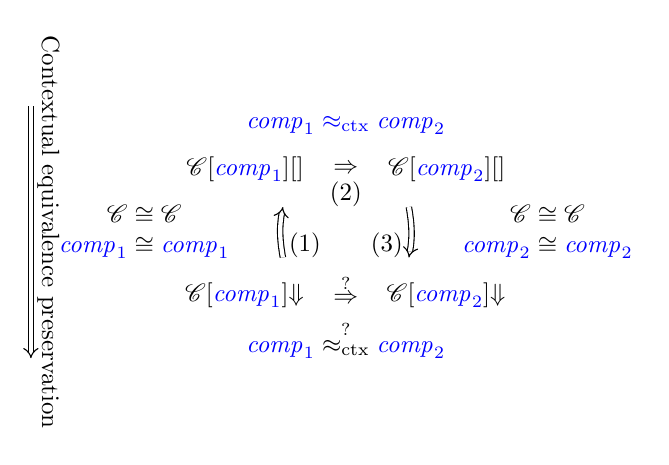
\begin{tikzpicture}[scale=0.8,every node/.style={scale=.9}]
    % \draw[help lines,yellow] (0,0) grid (10,7);
    \node at (5,4.7) { ${\src{\comp_1}\mathrel{\sconeq} \src{\comp_2}}$ };

    \node at (3.4,4) { ${\plug{\trg{\context}}{\src{\comp_1}} \sterm[]{\gc}{}}$ };
    \node at (5,4) { $\mathrel{\Rightarrow}$ };
    \node at (6.6,4) { ${\plug{\trg{\context}}{\src{\comp_2}} \sterm[]{\gc}{}}$ };

    \node at (4.35,2.8) { (1) };
    \node at (5,3.6) { (2) };
    \node at (5.65,2.8) { (3) };

    \draw[out=100,in=260,double,-implies,double equal sign distance] (4,2.6) to (4,3.4);

    \draw[out=280,in=80,double,-implies,double equal sign distance] (6,3.4) to (6,2.6);

    \node[align=center] at (8.2,3) { $ {\trg{\context}} \cong \trg{\context}$ \\
      $ {\src{\comp_2}} \cong {\src{\comp_2}}$};
    \node[align=center] at (1.8,3) { $ {\trg{\context}} \cong \trg{\context}$ \\
      $ {\src{\comp_1}} \cong {\src{\comp_1}}$};
    % \node at (9,2.7) { $e  {\src{C_1}} \cong \src{C_1}} : tau$ };
    % \node at (8.7,3.3) { $ {\trg{\context}} \cong \trg{\context} :{\emptyset},tau \ra e,{\cdots}$ };
    % \node at (.8,3) { $e  {\src{C_1}} \cong {\src{C_1}} : tau$ };

    \node at (3.4,2) { ${\plug{\trg{\context}}{\src{\comp_1}} \term[]{}}$ };
    \node at (5,2.1) { $\overset{?}{\Rightarrow}$ };
    \node at (6.6,2) { ${\plug{\trg{\context}}{\src{\comp_2}} \term[]{}}$ };

    \node at (5,1.3) { ${\src{\comp_1}}\mathrel{\overset{?}{\tconeq}}{\src{\comp_2}}$ };

    \draw[out=-90,in=90,double,-implies,double equal sign distance] (0,5) to node[sloped, yshift =.7em]{\Small Contextual equivalence preservation} (0,1);
  \end{tikzpicture}
  \caption{Proving one direction of fully abstract compilation (contextual equivalence preservation).}
  \label{fig:fa-proof-sketch}
\end{figure}


% \subsection{Proof sketch}
% \label{subsec:proof-sketch}
% \begin{proof}[Proof of Theorem~\ref{thm:full-abstraction}]
  % \item Consider first the upward arrow.
  %   Assume $\src{\var{comp}_1} \tconeq \src{\var{comp}_2}$.

  %   Take a $\src{\context}$ such that $\vdash \src{\context}$, take $\src{\ta[,i]}
  %   = \src{\dom(\var{comp}_i.\mscode)}$, $\gsigrets_i = \var{comp}_i.\sigrets$ and
  %   $\gsigcloss_i = \var{comp}_i.\sigcloss$, $\gc_i = (\ta[,i],\stkb_i,\gsigrets_i,\gsigcloss_i)$ and we will prove that
  %   $\src{\plug{\context}{\var{comp}_1} \sterm{\gc_1}} \Leftrightarrow
  %   \src{\plug{\context}{\var{comp}_2} \sterm{\gc_2}}$.

  %   By symmetry, we can assume w.l.o.g. that $\src{\plug{\context}{\var{comp}_1} \sterm{\gc_1}}$ and prove that $\src{\plug{\context}{\var{comp}_2} \sterm{\gc_2}}$.
  %   Note that this implies that $\src{\context}$ is a valid context for both $\src{\var{comp}_1}$ and $\src{\var{comp}_2}$.

  %   First, we show that also $\plug{\context}{\var{comp}_1} \trg{\term}$.
  %   Take $n$ the amount of steps in the termination of $\src{\plug{\context}{\var{comp}_1} \sterm{\gc_1}}$.
  %   It follows from Lemma~\ref{lem:ftlr-comps} that $\npair[n+1]{(\var{comp}_1,\var{comp}_1)} \in \lrcomp[\preceq,\gc_1](W_1)$ for some $W_1$ with $\dom(\pwfree) = \dom(\pwpriv) = \emptyset$.
  %   It also follows from the same Lemma~\ref{lem:ftlr-comps} that $\npair[n+1]{(\context,\context)} \in \lrcomp[\preceq,\gc_1](W_1')$ for some $W_1'$ that we can choose such that $W_1 \uplus W_1'$ is defined.
  %   Lemma~\ref{lem:compat-context-plug} then tells us that $\npair{(\plug{\context}{\var{comp}_1}, \plug{\context}{\var{comp}_1})} \in \lrec[\preceq,\gc_1](W_1\uplus W_1')$
  %   Together with $\src{\plug{\context}{\var{comp}_1} \sterm[n]{\gc_1}}$, Lemma~\ref{lem:adequacy} then tells us that $\plug{\context}{\var{comp}_1} \trg{\term}$.

  %   It follows from $\src{\var{comp}_1} \tconeq \src{\var{comp}_2}$ that also $\plug{\context}{\var{comp}_2} \trg{\term}$.

  %   It now remains to show that also $\src{\plug{\context}{\var{comp}_2} \sterm{\gc_2}}$.
  %   Take $n'$ the amount of steps in the termination of $\plug{\context}{\var{comp}_2} \trg{\term}$.
  %   It follows from Lemma~\ref{lem:ftlr-comps} that $\npair[n'+1]{(\var{comp}_2,\var{comp}_2)} \in \lrcomp[\succeq,\gc_2](W_2)$ for some $W_2$ with $\dom(\pwfree) = \dom(\pwpriv) = \emptyset$.
  %   It also follows from the same Lemma~\ref{lem:ftlr-comps} that $\npair[n'+1]{(\context,\context)} \in \lrcomp[\succeq,\gc_2](W_2')$ for some $W_2'$ that we can choose such that $W_2 \uplus W_2'$ is defined.
  %   Lemma~\ref{lem:compat-context-plug} then tells us that $\npair[n']{(\plug{\context}{\var{comp}_2}, \plug{\context}{\var{comp}_2})} \in \lrec[\succeq,\gc_2](W_2\uplus W_2')$
  %   Together with $\plug{\context}{\var{comp}_2} \trg{\term[n']}$, Lemma~\ref{lem:adequacy} then tells us that $\src{\plug{\context}{\var{comp}_2} \sterm{\gc_2}}$, concluding this direction of the proof.

%   First consider the right arrow:

%     Assume $\src{\var{comp}_1} \sconeq \src{\var{comp}_2}$. Take $\src{\ta[,i]} = \src{\dom(\var{comp}_i.\mscode)}$, $\gsigrets_i = \var{comp}_i.\sigrets$ and $\gsigcloss_i = \var{comp}_i.\sigcloss$, $\gc_i = (\ta[,i],\stkb_i,\gsigrets_i,\gsigcloss_i)$.
% %
%     Take a $\trg{\context}$ such that $\vdash \trg{\context}$ and we will prove that
%     $\trg{\plug{\context}{\var{comp}_1} \term} \Leftrightarrow
%     \trg{\plug{\context}{\var{comp}_2} \term}$.
% %
%     By symmetry, we can assume w.l.o.g. that $\trg{\plug{\context}{\var{comp}_1} \term}$ and prove that $\trg{\plug{\context}{\var{comp}_2} \term}$.
%     Note that this implies that $\trg{\context}$ is a valid context for both $\trg{\var{comp}_1}$ and $\trg{\var{comp}_2}$.
% %
%     First, we show that also $\plug{\context}{\var{comp}_1} \src{\sterm{\gc_1}}$.
%     Take $n$ the amount of steps in the termination of $\plug{\context}{\var{comp}_1} \trg{\term}$.
%     It follows from Lemma~\ref{lem:ftlr-comps} that $\npair[n+1]{(\var{comp}_1,\var{comp}_1)} \in \lrcomp[\succeq,\gc_1](W_1)$ for some $W_1$ with $\dom(\pwfree) = \dom(\pwpriv) = \emptyset$.
%     It also follows from the same Lemma~\ref{lem:ftlr-comps} that $\npair[n+1]{(\context,\context)} \in \lrcomp[\succeq,\gc_1](W_1')$ for some $W_1'$ that we can choose such that $W_1 \uplus W_1'$ is defined.
%     Lemma~\ref{lem:compat-context-plug} then tells us that $\npair{(\plug{\context}{\var{comp}_1}, \plug{\context}{\var{comp}_1})} \in \lrec[\succeq,\gc_1](W_1\uplus W_1')$
%     Together with $\plug{\context}{\var{comp}_1} \trg{\term[n]}$, Lemma~\ref{lem:adequacy} then tells us that $\plug{\context}{\var{comp}_1} \src{\sterm{\gc_1}}$.
% %
%     It follows from $\src{\var{comp}_1} \sconeq \src{\var{comp}_2}$ that also $\plug{\context}{\var{comp}_2} \src{\sterm{\gc_2}}$.
% %
%     It now remains to show that also $\plug{\context}{\var{comp}_2} \trg{\term}$.
%     Take $n'$ the amount of steps in the termination of $\plug{\context}{\var{comp}_2} \src{\sterm{\gc_2}}$.
%     It follows from Lemma~\ref{lem:ftlr-comps} that $\npair[n'+1]{(\var{comp}_2,\var{comp}_2)} \in \lrcomp[\preceq,\gc_2](W_2)$ for some $W_2$ with $\dom(\pwfree) = \dom(\pwpriv) = \emptyset$.
%     It also follows from the same Lemma~\ref{lem:ftlr-comps} that $\npair[n'+1]{(\context,\context)} \in \lrcomp[\preceq,\gc_2](W_2')$ for some $W_2'$ that we can choose such that $W_2 \uplus W_2'$ is defined.
%     Lemma~\ref{lem:compat-context-plug} then tells us that $\npair[n']{(\plug{\context}{\var{comp}_2}, \plug{\context}{\var{comp}_2})} \in \lrec[\preceq,\gc_2](W_2\uplus W_2')$
%     Together with $\plug{\context}{\var{comp}_2} \trg{\term[n']}$, Lemma~\ref{lem:adequacy} then tells us that $\plug{\context}{\var{comp}_2} \trg{\term}$, concluding the second direction of the proof.

%  The left arrow is proven in a similar manner.
% \end{proof}


\section{Discussion}
\label{sec:discussion}
% \begin{itemize}
% \item explain how fully abstract overlay semantics could form one pass of a verified secure compiler.
% \item Sharing stack references accross component boundaries is supported
% \item Other notions of well-bracketedness (specifically one would be to allow different stacks)
% \end{itemize}
\subsection{Full abstraction}
% - Full abstraction proofs difficult
Our formulation of WBCF and LSE using a fully abstract overlay semantics has an advantage with respect to others that we haven't discussed yet.
Imagine that you are implementing a fully abstract compiler for a high-level language, i.e.\ a secure compiler that enforces high-level abstractions when interacting with untrusted target-language components.
Such a compiler would need to perform many things and enforce other high-level properties than just WBCF and LSE.

If such a compiler uses the \stktokens{} calling convention, then the security proof should not have to reprove security of \stktokens{}.
Ideally, it should just combine security proofs for the compiler's other functionality with our results about \stktokens{}.
We want to point out that our formulation enables such reuse.
Specifically, the compiler could be factored into a part that targets \srccm{}, followed by our embedding into \trgcm{}.
If the authors of the secure compiler can prove full abstraction of the first part (relying on WBCF and LSE in \srccm{}) and they can also prove that this first part generates well-formed and reasonable components, then full abstraction of the whole compiler follows by our result and transitivity of fully abstract compilation.
Perhaps other reusable components of secure compilers could be formulated similarly using some form of fully abstract overlay semantics, to obtain similar reusability of their security proofs.

% When creating fully-abstract compilers between low-level machines, it is a big challenge to work with the exposed addresses.
% In particular, if the compilation changes the code size of a block of code, then it may be observable and prevent full-abstraction from being proven.
% We would argue that when a compilation reaches a phase where addresses are exposed, then the compilation should no longer change the code.
% This does, however, pose the challenge that there might quite a few abstractions in difference between the language where addresses are hidden to a machine where they are not.
% We propose that this challenge is solved by implementing these abstractions in a number of overlay semantics.
% By implementing them one by one, one can deal with one abstraction at a time reducing the complexity of each necessary full-abstraction proof.


% - Need to compile to a machine with enforcement mechanisms - capability machine an option
% - Full abstraction proofs modular, so other full abstraction proofs could target \srccm{} and thus have more abstractions to work with than if \trgcm{} was the target.

%\subsection{Sharing the stack}
% ?
\subsection{Practical applicability}
We believe there are good arguments for practical applicability of \stktokens{}.
The strong security guarantees are proven in a way that is reusable as part of a bigger proof of compiler security.
Its costs are
\begin{itemize}
\item a constant and limited amount of checks on every boundary crossing.
\item possibly a small memory overhead because every stack frame must be of non-zero length
\end{itemize}
The main caveat is that we rely on the assumption that capability machines like CHERI can be extended with linear capabilities in an efficient way.

Although this assumption can only be discharged by demonstrating an actual implementation with efficiency measurements, the following notes are based on private discussions with people from the CHERI team as well as our own thoughts on the matter.
As we understand it, the main problems to solve for adding linear capabilities to a capability machine like CHERI are related to the move semantics for instructions like \texttt{move}, \texttt{store} and \texttt{load}.
Processor optimizations like pipelining and out-of-order execution rely on being able to accurately predict the registers and memory that an instruction will write to and read from.
Our instructions are a bit clumsy from this point-of-view because, for example, \texttt{move} or \texttt{store} will zero the source register resp. memory location if the value being written is linear.
A solution for this problem could be to add separate instructions for moving, storing and loading linear registers at the cost of additional opcode space.
Adding splice and split will also consume some opcode space.

Another problem is caused by the move semantics for \texttt{load} in the presence of multiple hardware threads.
In this setting, zeroing out the source memory location must happen atomically to avoid race conditions where two hardware threads end up reading the same linear capability to their registers.
This means that a \texttt{load} of a linear capability will need to behave like an atomic operation similar to a compare-and-swap instruction.
This is in principle not a problem except that a compare-and-swap is significantly slower than a regular \texttt{load} (on the order of 10x slower or more).
When using \stktokens{}, loads of linear capabilities normally happen only when a thread has stored its return data capability on the stack and loads it back from there after a return.
Because the stack is a region of memory with very high thread affinity (no other hardware thread should access it, in principle), and which is accessed quite often, we are hopeful that well-engineered caching could reduce the high overhead of atomic loads of linear capabilities.
If such memory could be (mostly) kept exclusively locked in a cache close to the processor, the overhead of atomic loads in \stktokens{} might be significantly less than \texttt{load}'s worst case.
The processor could perhaps also (be told to) rely on the fact that race conditions should be impossible for loads from linear capabilities (which should in principle be non-aliased) and just use a non-atomic load in that case.

\section{Related Work}

\todo{Watson et al.\ (XXX: fix name to reflect citation) have concurrently developed an extension of the CHERI-MIPS instruction set with linear capabilities.}
\todo{\url{https://nakamotoinstitute.org/scarce-objects/}}
\todo{\url{http://journals.uic.edu/ojs/index.php/fm/article/view/548}}

In this section, we discuss related work on securely enforcing control flow correctness and/or local state encapsulation.
We do not repeat the work we discussed in Section~\ref{sec:introduction}.

Capability machines originate with \citet{dennis_programming_1966} and we refer to \citet{levy_capability-based_1984} and \citet{watson_cheri:_2015} for an overview of previous work.
The capability machine formalized in Section~\ref{sec:cap-mach-w-seal-and-lin} is modelled after CHERI~\citep{watson_cheri:_2015,woodruff_cheri_2014}.
This is a recent, relatively mature capability machine which combines capabilities with a virtual memory approach in the interest of backwards compatibility and gradual adoption.
For simplicity, we have omitted features of CHERI that were not needed for \stktokens{} (e.g.\ local capabilities, virtual memory).

Plenty of other papers enforce well-bracketed control flow at a low level but most are restricted to preventing particular types of attacks and enforce only partial correctness of control flow.
This includes particularly the line of work on \emph{control-flow integrity}~\citep{abadi_control-flow_2005}.
This technique prevents certain classes of attacks by sanitizing addresses before direct and indirect jumps based on static information about a program's control graph and a shadow stack.
Contrary to \stktokens{}, CFI can be implemented on commodity hardware rather than capability machines.
However, its attacker model is different, and its security goals are weaker.
They assume an attacker that is unable to execute code but can overwrite arbitrary data at any time during execution (to model buffer overflows).
In terms of security goals, the technique does not enforce local stack encapsulation.
Also, it only enforces a weak form of control flow correctness saying that jumps stay within the static control flow graph of a program~\cite{Abadi2005Theory}.
Such a property ignores temporal properties and seems hard to use for reasoning.
There is also more and more evidence that these partial security properties are not enough to prevent realistic attacks in practice~\citep{Evans:2015:CJW:2810103.2813646,Carlini2015ControlFlowBending}.

More closely related to our work are papers that use separate per-component stacks, a trusted stack manager and some form of memory isolation to enforce control-flow correctness as part of a secure compilation result~\citep{patrignani_modular_2016,juglaret_beyond_2016}.
Our work differs from theirs in that we use a different low-level security primitive (a capability machine with local capabilities rather than a machine with a primitive notion of compartments), and we do not use per-component stacks or a trusted stack manager but a single shared stack and a decentralized calling convention based on linear capabilities.
Both prove a secure compilation result from a high-level language which clearly implies a general form of control-flow correctness, but that result is not separated from the results about other aspects of their compiler.

CheriBSD applies a similar approach with separate per-component stacks and a trusted stack manager on a capability machine~\cite{watson_cheri:_2015}.
The authors use local capabilities to prevent components from accidentally leaking their stack pointer to other components, but there is no actual capability revocation in play.
They do not provide many details on this mechanism and it is, for example, not clear if and how they intend to deal with higher-order interfaces (C function pointers) or stack references shared across component boundaries. 

The fact that our full abstraction result only applies to reasonable components (see Section~\ref{sec:form-secur-with}) makes it related to full abstraction results for unsafe languages.
In their study of compartmentalization primitives, \Citet{juglaret_beyond_2016} discuss the property of Secure Compartmentalizing Compilation (SCC): a variant of full abstraction that applies to unsafe source languages.
Essentially, they modify standard full abstraction so that preservation and reflection of contextual equivalence are only guaranteed for components that are {\itshape fully defined}, which means essentially that they do not exhibit undefined behavior in any fully defined context.
In follow-up work, \citet{abate_good_components_2018} extend this approach to scenarios where components only start to exhibit undefined behavior after a number of well-defined steps. 
If we see reasonable behavior as defined behavior, then our full abstraction result can be seen as an application of this same idea.
Our results do not apply to dynamic compromise scenarios because they are intended to be used in the verification of a secure compiler where these scenarios are not relevant.

\begin{acks}
  This work was supported by Cost Action CA15123 EUTypes.
  Dominique Devriese held a Postdoctoral Fellowship from the Research Foundation - Flanders (FWO) during most of this research.
\end{acks}

\bibliography{references}


%% Appendix
% \appendix
% \section{Appendix}

% Text of appendix \ldots

\end{document}
 